%todo:


% mh 7/19
% in experiment 1 and model, take the speaker perspective when talking about how the model works




%from noah 1/30 am:
%-add some more points to the x axis in figure 6 so the mosquitos prior looks bimodal. perhaps show as curves instead of bars?


% - get tiny URLs for experiment links
% - set up forest page
% - fit into space and proof read.


% - if time: look at "order effect" in prior elicitation (taboo sampling hypothesis... first sample is 0, second is 100, third - fifth are meh)
% - make figures 1 & 2 as pretty as 3 & 4




% - try rationality parameter in tfbt model
% - look at "order effect" in prior elicitation (taboo sampling hypothesis... first sample is 0, second is 100, third - fifth are meh)
% - do we really want posterior predictives that include the guessing parameter? (the guessing parameter is part of the analysis model, not the cognitive model...)
%- what kind of evidence do we want to use at the end to relate inferred priors to elicited? 
%	- is eye-balling the elicited prior and the mean inferred priors sufficient?
%	- i tried TFBT on the elicited priors to back out gamma & deltas, but gammas don't seem to come apart for DD vs. plain (as they do in the inferred priors from Exp 1 &2)
%	- one possible way to get this sort of "ordered gammas" evidence would be to repeat the prior elicitation with more items per trial
%		- the thought is that in our prior elicitation, i used 5 animals per slide (and 6 trials)
%			- probably there was not enough dynamic range for Plain vs DD to come apart 
%		- i think with 10 items, it would be better (but does that mean just 3 trials, one in each context, per subj?) [there are only 30 animals]
%% --- not sure if the above comments about prior elicitation still hold with the fixed TFBT model, but Noah's suggestion was for 1 animal at a time

%		
%todo after cogsci:
%-run additional contexts. e.g. separate dangerous and distinct.
%-look again at finer-grained truth judgement task?
%-think about the weird cases of generics in the literature. e.g. ``robins lay eggs''.
% - try an S2 model of prevalence judgement task, too. does it reduce to the L1 model?

%


% comments from workshop class 4/29
%
% why spend a lot of time in replication?
% 7 --- summary sentence 2nd paragraph to intro
% abstract worrisome
% look at study discussions -- move stuff to intro
%
% Lay eggs vs. Are female /// John is tall vs. ESB is tall [move even earlier]
% Move "a natural foil" earlier
%
% Maybe add talk of stereotypes?
% Craig: Use speaker / listener actors more; think about the person and the thing they're doing
% 
% Simulations of theoretical analysis: first sentence WHOA
%
%  beef up penultimate paragraph in intro: talk about why distinctive and dangerous are important
% ---- unpack distinctive and dangerous (use experimental materials)
%
% TABLE for materials and experiment. 
% maybe set up replication-idea early.  and then go on.




% details
%
% Section 4: exp 2 intro
%% oceans underneath each sentence
%% connect back with behavior--- asymmetry, truth cond
%
% pre Exp 3: use 
% "endemic to the entire category"
% exp3a: jargon word 
% (reuse penultimate intro paragraph throughout) [maybe make higher level version of this paragraph for intro]
%
% pre-experiments, "Like Exp 2c, 3b did BLAH but differed "
%
% add more to figure captions?
%
%
% seeds of very last paragraph in earlier
%
% in conclusion: what do the tools allow us to do? (e.g. w/ stereotyping) 
% differences in prior knowledge --> how does this contribute to language change?
% 




\documentclass[10pt,letterpaper]{article}
% Default margins are too wide all the way around. I reset them here
%\setlength{\topmargin}{-.5in} \setlength{\textheight}{9in}
%\setlength{\oddsidemargin}{.125in} \setlength{\textwidth}{6in}

\usepackage{setspace}
\doublespacing

\usepackage{geometry}
\geometry{legalpaper, margin=1in}

\usepackage{pslatex}
\usepackage{apacite}
\usepackage{url}
\usepackage{graphicx}
\usepackage{caption}
\usepackage{subcaption}
\usepackage{listings}
\usepackage{color}
\usepackage{textcomp}
\usepackage{amsmath}
\usepackage{amssymb}
\usepackage{wrapfig}
\usepackage{lipsum}

\graphicspath{{figures/}}

\def\signed #1{{\leavevmode\unskip\nobreak\hfil\penalty50\hskip2em
  \hbox{}\nobreak\hfil(#1)%
  \parfillskip=0pt \finalhyphendemerits=0 \endgraf}}

\newsavebox\mybox
\newenvironment{aquote}[1]
  {\savebox\mybox{#1}\begin{quote}}
  {\signed{\usebox\mybox}\end{quote}}


 \newcommand{\denote}[1]{\mbox{ $[\![ #1 ]\!]$}}


%\lstset{
%  language=Scheme, % Andreas Stuhlmuller. Scheme listings. https://github.com/stuhlmueller/scheme-listings.git
%  columns=fixed,
%  tabsize=2,
%  extendedchars=true,
%  breaklines=true,
%  frame=single,
%%  numbers=left,
%  numbersep=5pt,
%   basicstyle=\scriptsize\ttfamily
%%  rulesepcolor=\color{solarized@base03},
%%  numberstyle=\tiny\color{solarized@base01},
%%  keywordstyle=\color{solarized@green},
%%  stringstyle=\color{solarized@cyan}\ttfamily,
%%  identifierstyle=\color{blue},
%%  commentstyle=\color{solarized@base01},
%%  emphstyle=\color{solarized@red}
%}

\definecolor{Red}{RGB}{255,0,0}
\newcommand{\red}[1]{\textcolor{Red}{#1}}  

\usepackage{titlesec}

\setcounter{secnumdepth}{4}

\titleformat{\paragraph}
{\normalfont\normalsize\bfseries}{\theparagraph}{1em}{}
\titlespacing*{\paragraph}
{0pt}{3.25ex plus 1ex minus .2ex}{1.5ex plus .2ex}



%\title{Words are vague: A prevalence-based account of generic language}
\title{Generic language is vague yet rationally / pragmatically understood}
% \title{Generic statements are vague}
% \author{{\large \bf Michael Henry Tessler, Noah D. Goodman } \\
%	\{mhtessler, ngoodman\}@stanford.edu \\
%  Department of Psychology, Stanford University}

\author{{\large \bf Michael Henry Tessler} (mtessler@stanford.edu)\\ {\large \bf Noah D. Goodman} (ngoodman@stanford.edu) \\
  Department of Psychology, Stanford University}
 
\begin{document}
%\newpage
%\tableofcontents
%\newpage
%\listoffigures
%\newpage
\maketitle


\begin{abstract}
Generic utterances (e.g. ``Dogs bark'') express ideas about categories in the world and are ubiquitous in everyday conversation. 
Despite their prevalence, the meanings of generic statements are puzzling to formal theories. 
It is believed that generic utterances behave somewhat like quantified ones (e.g. ``Most dogs bark.''). 
If this is correct, however, there should be some threshold on the percentage of the category that must display the property (e.g. some criterion number of dogs that bark) for the utterance to be true.
This threshold is notoriously difficult to define for generics, which are flexible enough to be true based on very little evidence while also implying near-universality of the property. 
Here, we formalize a semantics and pragmatics for generic language understanding, based on the idea that generics are vague: The threshold for acceptance is represented as an unknown property of the language and is actively reasoned about in context by a listener who assumes she is in conversation with an informative speaker. 
We explain how this simple semantics can account for two central phenomena surrounding generic language: The flexible conditions by which a generic is true and the variable implications of generic language. 
Inferences from the model are driven largely by the listeners' \emph{a priori} beliefs about the property, which we measure empirically.
%We predict human acceptability judgments and interpretations of generics of both familiar and novel categories with strong quantitative accuracy using a novel behavioral and data-analytic technique for measuring beliefs about the prevalence of properties coupled with our model of generic language. 
This work suggests that the semantics of generic statements can treated as scalar and that listeners' expectations in the form of prior beliefs heavily govern generic interpretation. 

%To illustrate the model, we measure participants' expectations about the prevalence of certain properties in addition to the acceptability of a number of generic utterances. 
%We show %how prevalence alone cannot account for truth judgments of the associated generic statements, but
%how a simple vague semantics, coupled with listeners' prior expectations about the property and basic conversational principles can explain the puzzlingly wide array of conditions by which a generic is true.
%more elaborate account based on distributions of prevalence and conversational principles can. 
%A second puzzle surrounds interpretations of generic utterances. Though accepted for a range of prevalences,  generics are often interpreted as applying to nearly all of the category. 
%We replicate and extend an experimental finding validating this intuition and show how the vague, prevalence-based model predicts this asymmetry between truth judgments and interpretations. 

%We illustrate the model by showing its ability to capture gender-specific and low-prevalence generics---two cases of theoretical importance
%We replicate two major previous findings: (1) Generics about dangerous or distinctive properties are more acceptable than similar generic statements such connotations, and (2) Novel generic statements (e.g. ``Lorches have purple feathers) are interpreted as applying to nearly all of a category (i.e. almost all lorches have purple feathers) while the same statements are accepted as true for a wide range of prevalence levels (e.g. when only 10\% of lorches have purple feathers). The prevalence-based model predicts (1) [differential acceptability of generics] if the prior distribution over the prevalence (i.e. the probability of the property given the category) differs between these different types of properties. The prevalence model also predicts (2) [strong implications of generic] if the prior over prevalence is bimodal with a peak at 100\%. We find direct evidence that this is so by eliciting the prior distribution over prevalence empirically. 
%
%
%Here, I formalize a prevalence-based
%semantics, wherein the threshold for acceptance is represented as an unknown
%property of the language, and must be actively reasoned about in context by the
%listener. I will illustrate this model by showing its ability to capture gender-specific
%and low-prevalence generics---two cases of theoretical importance. I?ll go on to show
%how this model can account for previous empirical findings that (1) Generics about
%dangerous and distinctive properties are more acceptable than similar generic
%statements lacking such connotations, and (2) Novel generic statements (e.g.
%?Lorches have purple feathers?) are interpreted as applying to nearly all of a
%category (i.e. almost all lorches have purple feathers) while the same statements are
%accepted as true for a wide range of prevalence levels (e.g. when only 30% of
%lorches have purple feathers). I?ll try to conclude by discussing future directions of
%this work relating to the pragmatics of experimental contexts.


%demonstrated that the endorsement rate of generic statements differs by context, and that generics can be endorsed based on weak evidence while the same sentences are interpreted strongly. Here, we replicate these effects in Exp.~1 and investigate how models based on prevalence (the probability of the property given the category) can account for this behavior. 
%Using Bayesian data analysis techniques, %to make inferences about the putative threshold used as well as to arbitrate between competing accounts. 
%we show how a simple scalar prevalence semantics is untenable, but that the same semantics within a probabilistic pragmatics framework can account for the data. 
%In this model, the generic has an underspecified meaning, but this uncertainty is resolved by context and interaction. 
%Context effects are predicted if the prior distribution of prevalence differs by context; in Exp.~2 we find direct evidence that this is so.
%The differences between verification and interpretation are understood as different tasks within a communicative framework. 
%We use a Bayesian analysis again to infer a prior distribution, for which we then find confirmatory evidence in Exp. 2. 


\textbf{Keywords:} 
generics; probabilisitic pragmatics
\end{abstract}

%\begin{aquote}{John Locke, \emph{An Essay Concerning Human Understanding (1690)}}
%Now since [articulate] sounds have no natural connexion with our ideas, but have all their signification from the arbitrary imposition of men, the doubtfulness and uncertainty of their signification has its cause more in the ideas they stand for than in any incapacity there is in one sound more than in another to signify any idea: For in that regard they are all equally perfect.
%\end{aquote}


%Imagine talking with a 3-year-old about engines. Engines are difficult to explain because they are so often observed when they are unobserved as when they are hidden beneath a car's shell. You might say, ``Engines turn gas into energy, and that makes cars go''. Few would argue with the truth of this sentence, yet its meaning is difficult to specify. 
%
% is so rarely observable and the function of oxygen is abstract. 
%You might offer, ``Animals breathe oxygen to live.''. 
%Few would argue with the truth of this sentence, yet its meaning is difficult to specify. 


Imagine talking with a 3-year-old about oxygen. Oxygen is difficult to explain because it is so rarely observable and the function of oxygen is abstract. 
You might offer, ``Animals breathe oxygen to live.''. 
Few would argue with the truth of this sentence, yet its meaning is difficult to specify. 

%Is it synonymous with ``All animals breathe Oxygen to live''? %It's false that \emph{all} animals breathe oxygen (e.g. fish), yet intuitively the sentence seems to convey something stronger than the weak \emph{some} animals breathe oxygen. 
%If you were talking with an adult, you might use a more nuanced statement (e.g. by talking about the subcategory Mammals).
%Words are vague because ideas are vague, Locke argues. In making this argument, he falls into the habit of communication that we all fall into: using generalizations about members of a category---in this case, \emph{[articulate] sounds}. 
%
This type of utterance is generic \cite{Carlson1977, Leslie2008} in that it conveys a generalization about a category (e.g. \emph{animals}).  
Generics are one of the simplest linguistic constructs. 
They have no explicitly marked operator and yet children as young as two or three can correctly understand that they refer to categories and not just a plurality in a scene \cite{Cimpian2008}. 
Generics are ubiquitous in everyday conversation as well as in child-directed speech \cite{Gelman2008} and are thought to be essential to the growth of conceptual knowledge \cite{Gelman2004}. 
At the same time, generics are the primary vehicle by which stereotypes are conveyed \cite{GelmanEtAl2004, Cimpian2010motivation, Leslie2015}.
Despite their centrality to cognitive development and everyday conversation, generic utterances have elusive meanings. % stable meanings for generic sentences are hard to come by.

The semantics of generics is often contrasted with that of quantifier sentences, which are commonly understood in terms of the prevalence of a property and are straightforward to evaluate for truth. 
For example, for ``\emph{Some} animals breathe oxygen.'' to be true, then there must be at least one animal that does so. 
``\emph{Most} animals breathe oxygen.'' is true because more than half do. 
``\emph{All} animals breathe oxygen.'' is actually not true because there are three species of creatures called \emph{lorica} that live 2.2 miles underwater on the ocean floor in an oxygen-free environment \cite{Danovaro2010}; ``all'' means 100\%. 
%then there really can be no exceptions: 100\% of animals must breathe oxygen for the sentence to be valid. 
But what about ``Animals breathe oxygen.''? 
Is there some prevalence beyond which the generic becomes true?

Prevalence based accounts are difficult to defend. 
At first glance, generics seem like universally-quantified statements (i.e. ``All animals breathe oxygen''), but generics are resilient to counter-examples like \emph{lorica}. 
Interpreting the generic as meaning ``most'' captures many cases, but cannot explain why ``Robins lay eggs'' and ``Mosquitos carry West Nile Virus'' both seem true, despite the fact that only adult female robins lay eggs and that less than 1\% of mosquitos actually carry West Nile Virus. 
The only quantifier that could satisfy all of these conditions is the weak ``some''.  
Yet, the semantics for ``some'' cannot be the semantics of generics:  Upon hearing a generic, listeners are wont to interpret the sentence as applying to \emph{all or nearly all} of a category \cite{Gelman2002, Cimpian2010}. 
``Some animals breathe oxygen'' does not carry the same generalizability.

%This flexibility in meaning poses a challenge for linguists and philosophers, but seemingly little trouble for the language learner. Three-year-olds can use pragmatic cues to recognize generics as referring to instances beyond those in a particular scene \cite{Cimpian2008}. Preschoolers have adult-like interpretations of novel generic sentences about both familiar and unfamiliar categories \cite{Gelman2002, Brandone2014}. Finally, generics are ubiquitous in child-directed speech, being both produced by the caregiver and the child from age two \cite{Gelman2008}. The meaning of generic sentences are hard to pin down formally, yet children seem to master the relevant interpretative skills at a very young age.
%
%You might think, then, that generics are synonymous with weaker ``most''-statements. However, we'll only be able to maintain this logic until we encounter generics like ``Birds lay eggs'' or ``Mosquitos carry West Nile Virus'', which are both intuitively true despite the fact that only adult female birds lay eggs and that less than 1\% of mosquitos carry West Nile Virus. The only quantifier that could satisfy all of these conditions is the existential ``some''.  Yet, the semantics for ``some'' cannot be the semantics of generics:  Upon hearing a generic, listeners are wont to interpret the sentence as applying to \emph{all or nearly all} of a category \cite{Gelman2002, Cimpian2010}. ``Some animals breathe oxygen'' implies something quite different (e.g. that \emph{not all} animals breathe oxygen) \cite{Degen2015}.


% Generics can be true based on very little evidence (e.g. each of us has encountered only a small number of all the animal-kinds in the world). % should I deply the mosquitos here?
%
%is making his argument not based on a corpus study of words but based on his intuition and the particular examples he is considering implicitly, a relatively small proportion of the potential infinitude of articulate sounds. 
%
%At the same time, generics are robust to counterexamples
%
%Locke's argument is still tenable even if we know that we know there are non arbitrary word--meaning mappings (hence, ``\emph{all} sounds have no natural connexion with our ideas'' is false, \red{cite bouba-kiki, erin?, molly?}). 
%
%Finally, generics have strong implications.%

What could be the stable meaning of a generic given this extreme flexibility? 
We propose these phenomena can be explained as the effects of pragmatic inference filling in a meaning that is underspecified in the language. 
%
 %We propose that the meaning of a generic is underspecified in the language and these phenomena can be explained as the effects of pragmatic inference over this underspecified meaning. %
 %
In particular, we posit that generics are a vague description of prevalence in much the same way that gradable adjectives like \emph{tall} are vague descriptions of height. 
To understand the vagueness of ``tall'', consider the conditions by which a person is ``tall'' versus the conditions for a building to qualify as ``tall''.
This context-sensitivity of meaning can be accounted for by treating the condition for tallness (i.e. the threshold beyond which something counts as tall) as an unknown property of the language, and modeling the listener as inferring this threshold in context \cite{Lassiter2015}. 
The fact that the distributions of heights for buildings and people are different, and that listeners expect speakers to be truthful and informative \cite{Clark1996, Grice1975, Levinson2000}, produces intuitive meanings for vague adjectives.
 
%In a similar way, we posit a simple, scalar semantics for generics in which they express that the probability of the property given the kind-----i.e. the property's \emph{prevalence}-----is above a threshold (cf. \citeA{Cohen1999}). Following \citeA{GoodmanLassiter}, we treat this threshold as unknown property of the language and thus, as a variable that must be reasoned about in context. In this way, generics are vague in the way gradable adjectives like ``tall'' are vague: There is inherent uncertainty in the words' context-independent meaning. In this extension of the \emph{Rational Speech-Act} (RSA) framework \cite{Frank2012,Goodman2013}, the listener is tasked with the joint problem of figuring out what the speaker intended to communicate as well as what the generic means \emph{in this context}. 

In a similar way, we posit a simple, scalar semantics for generics in which they express that the probability of the property given the category-----i.e. the property's \emph{prevalence}-----is above a threshold (cf. \citeA{Cohen1999}). We treat this threshold as unknown property of the language and thus, as a variable that must be reasoned about in context. 

It might seem paradoxical that vague language should get so much usage. 
Shouldn't speakers want to express their ideas as clearly as possible?
Language evolutionary pressures suggest that, to the contrary, such underspecification is in fact useful, given that there is some context through which the uncertainty can be resolved \cite{Piantadosi2012}.
In this work, context takes the shape of a listener and speaker's shared beliefs (i.e. common ground) about the property in question. This, coupled with 
%With uncertainty in the language, the listener figures out what the words mean by drawing upon her prior beliefs---in this case about the prevalence of the property---in addition to harnessing 
standard inferences from conversational pragmatics, allows the listener to figure out the meaning of the otherwise vague utterance.
We extend the \emph{Rational Speech-Acts} (RSA) framework \cite{Frank2012,Goodman2013} to consider how a speaker determines what generics are acceptable to produce and how a listener might interpret generics differently depending on her belief's about the property in question. 
This formalism gives a new, computational perspective on how ideas are conveyed and how beliefs play a central role in understanding language.

% tasked with the joint problem of figuring out what the speaker intended to communicate as well as what the generic actually means \emph{in a context}. 

%This model predicts the degree to which a given generic utterance will be acceptable, and predicts how this might vary for different types of properties. 
%The vagueness simultaneously gives rise to variable interpretations contingent on the listener's beliefs about the distribution of the property. 
%We show how these predictions are borne out in a series of experiments.
%
\subsection{The phenomena}

One important test for a theory of generic meaning is that it captures the intuition shared by language users about the truth of certain generic sentences. To test the predictions of this model, we must first measure participants' prior expectations about the prevalence of the properties in question. Critically, however, we must measure not only prior expectations about the prevalence of the property for the category \emph{alone} but the distribution of expectations across categories (i.e. not only the probability of laying eggs for a robin, but also the probability of laying eggs for a cow and other animal species).  
We show how prevalence within the category alone is insufficient to explain generic acceptability, but a model that reasons pragmatically about the distribution over prevalence is sufficient to explain the variability in truth judgments.

Generic statements are not only puzzling because of their variable truth conditions, but also because of how they are interpreted. \citeA{Gelman2002} found that listeners  interpret novel facts about animals in the form of generics (e.g. ``Bears like to eat ants.'') as applying to nearly all of the category. Interpretations of bare plurals of novel animals with accidental properties (e.g. ``Morseths have wet fur.'') were found to be much weaker \cite{Cimpian2010}. These differences in interpretation are thought to be a result of different beliefs about the properties in question. This intuition is readily formalized in our language understanding model. Beliefs about properties are measured in independent experiments to serve as a foundation for the model's predictions. 
We compare our model's predictions to experiments examining the acceptability of naturalistic generics and interpretations of generics about novel categories.

%\citeA{Cimpian2010} employed a paradigm to assess the relationship between the \emph{truth judgments} and \emph{interpretations} of novel generic statements. In these studies, the \emph{interpretations} of generic statements were measured by asking participants to report the prevalence of the property within the category upon hearing the associated generic, e.g. ``Lorches have purple feathers. What \% of lorches do you think have purple feathers?'' In this task, subjects reported that almost all of the category had the property (i.e. almost all lorches have purple feathers.). In the \emph{truth judgments} task, participants were given prevalence information (e.g. ``30\% of lorches have purple feathers.'') and asked if the associated generic statement (i.e. ``Lorches have purple feathers'') was true or false. The results suggest an apparent ``paradox'' in the form of an asymmetry between the truth judgments of generics and the interpretations of generics:  Generics are accepted at prevalence levels as low as 10\%, but are interpreted as applying to nearly 100\% of the category\footnote{This asymmetry was absent for the sentences that used the quantifier ``most'', arguably the quantifier with the most similar meaning to generics \red{[cite]}}.  In a follow-up experiment, the authors showed how the interpretations of generics can be greatly weakened if the property in question is not a biological property (e.g. ``purple feathers'') but instead an accidental property (e.g. ``muddy feathers''). We replicate these findings and show how the apparent ``paradox'' can be explained by the interaction of an uncertain semantics with a prior distribution over the prevalence of biological properties. We further show how the interpretations of generics can be substantially weakened when the listener considers the distribution of prevalence for accidental properties.

%
%We demonstrate that the model captures cases of theoretical importance: gender-specific and low-prevalence generics. We replicate the main effects reported by \citeA{Cimpian2010} and use Bayesian data analytic techniques to further examine how the effective truth conditions of generic statements interact with the prior on prevalence. We show that our model predicts both flexible truth conditions and asymmetry effects, given appropriate priors over prevalence (``\emph{backward predictions} of the model''). We experimentally elicit the prevalence priors in CBG's experimental contexts, verifying these predictions (Expt.~2). We show that the elicited prevalence priors predict the same effects as the inferred priors (``\emph{forward predictions} of the model''), and then show how the effects dissipate when different types of properties (with different types of priors) are discussed (Expt.~3). Finally, we explore a case when the flexibility of truth conditions are difficult to associate with prevalence (Expt.~4). 


%\subsection{Previous findings}
%Determining the truth of individual generic statements is typically left to the intuitions of linguists \cite{Carlson1977, Leslie2008}. Psychological investigations have provided a complementary avenue to understanding the meaning of generic language by controlling for	various intrinsic differences between the examples considered by linguists. \citeA{Cimpian2010} carried out a series of experiments designed to examine the acceptability and implications of generic statements about novel animal categories (e.g.~``Lorches have purple feathers'') . 
%They found evidence that if the property in question was dangerous (e.g. ``These feathers are as sharp as needles and can easily get lodged in you, causing massive bleedings.'') or distinctive (e.g. ``No other animals have these kinds of feathers.''), the associated generic (i.e. ``Lorches have purple feathers'') was endorsed more and at lower prevalence levels (e.g. when only 10\% of lorches had purple feathers). This finding suggests that the conditions under which a generic is true---the generic's \emph{truth conditions}---vary as a function of the type of property being discussed (e.g. a dangerous property, a distinctive property). Distinctive properties are theoretically interesting because they intuitively map onto naturally-occurring generic statements that participant's readily endorse (e.g. ``Birds lay eggs'', ``Cardinals have red feathers''). In a similar vein, dangerous properties are intriguing because the truth conditions of such generic statements seem to be divorced from the prevalence of the property as in ``Mosquitos carry West Nile Virus'' ($<$ 1\% of mosquitos carry the virus) and ``Sharks attack swimmers''.
%
%\citeA{Cimpian2010} used a complementary task to assess the \emph{implications} of generic statements. In these studies, the \emph{implications} of generic statements were measured by asking subjects prevalence questions, e.g. ``What \% of lorches do you think have purple feathers?'' In this task, subjects reported that almost all of the category had the property (i.e. almost 100\% of lorches have purple feathers.). This raises an apparent asymmetry between the truth conditions of generics (generics are accepted at prevalence levels as low as 10\%) and the implications of generics (generics are interpreted as applying to nearly 100\% of the category). 

%\subsection{The current investigations}


%The asymmetry effects fall out of modeling task differences between the language understanding and answer-selection tasks faced by participants in the different experiments (cf. \citeA{Degen2014}). 
%Presumably, Locke is arguing about \emph{almost} all words. Why else would he go through the trouble of crafting this argument?
%
%\red{
%In this paper, we will see that the \emph{context} in which his words are uttered is essential to the meaning we derive. We propose that this aspect of generic language follows from pragmatic reasoning about an uncertain threshold for meaning; an idea which we formalize in a probabilistic model within the Rational Speech Acts framework \cite{Frank2012,Goodman2013}.
%%
%Generic statements are puzzling because their meaning is so flexible. On the one hand, generics would seem to suggest an almost universal quantification, as in ``Dogs bark''. Others, like ``Mosquitos carry West Nile virus'', involve a property that applies only to a small subset of the kind. 
%}
%It is perhaps this inherent uncertainty that leads generics to be so widespread in natural language. 


 %suggested that different dependent measures in experimental pragmatics paradigms map onto different communicative roles, and thus should be modeled accordingly. 

%We draw on new advances in probabilistic pragmatics to formalize two possible theories of the generic. Further, we harness the power of Bayesian data analysis to mediate between these formal theories and draw inferences about cognitively interesting model parameters. 


%(e.g. ``These feathers are as sharp as needles and can easily get lodged in you, causing massive bleeding. No other animals have these kinds of feathers'')
% (e.g.  ``These feathers are wide and very smooth to the touch. Other animals have these kinds of feathers.'')

%How are we to understand these data? One interpretation is that context changes the truth-conditions for a generic statement, but that within a context, the truth-conditions are stable. A different sort of explanation is that context changes the nature of world somehow, and that generic meanings are inferred rationally from context. We draw on recent advances in probabilistic pragmatics and Bayesian data analysis to mediate between these two alternatives.

\section{A lifted-threshold model of generic meaning}
\label{sec:model}

The meanings of words are often embedded in a conversational context.
Language understanding is a special case of social cognition---interlocutors think about one another when producing and interpreting utterances.  
Recent work in probabilistic pragmatics formalizes how listeners arrive at rich interpretations of utterances by considering the thought-processes of a speaker whose goal is to be informative.
The Rational Speech-Act (RSA) theory of language understanding \cite{Frank2012, Goodman2013} has provided formal, computational accounts of understanding utterances with quantifiers \cite{Goodman2013}, gradable adjectives \cite{Lassiter2015}, and nonliteral usages \cite{Kao2014}.

%Variants of this theory have provided formal explanations for a number of linguistic phenomena including scalar implicature, hyperbole, and argument evaluation \cite{Kao2014, Tessler2014, Lassiter2014}. 

%CBG showed how contexts affects the endorsement for generic statements. An additional concern of their experiments surrounded the relation between two dependent measures for understanding generics. One dependent measure was the ``truth conditions'', or \emph{sentence verification} measure that we've been considering up to this point. The other was an ``implied prevalence'', or \emph{sentence interpretation} dependent measure. The latter was collected by giving participants the generic statement (plus, any additional contextual information), and asking the participant ``What percentage of lorches have purple feathers?''

%The tasks in Exp.~1 are, fundamentally, language understanding tasks. Participants are given premises and asked to draw a conclusion that necessarily involves reasoning about the meaning of words. 

%\subsection{Lifted-variable RSA}

%The Bayesian data analysis above provides compelling evidence that context influences the truth-conditions of a generic statement. The poor qualitative fit as well as the high inferred value of the guessing parameter $\phi$ suggest, however, that our language model is incomplete. Rather than propose that the meaning of a generic is simply a one-to-one mapping between context and threshold, 

Recently, the Rational Speech-Act theory has been extended to account for gradable adjectives like \emph{tall}, which lack single, context-invariant meanings. 
This is done by positing the semantics of the word (``tall'') is a distribution over criteria (``anything could count as tall given the right context''). 
This uncertainty is resolved through a listener consulting her beliefs about the domain in question (``what are probable heights of a person?'') as well as taking into account the communicative force of a speech act (``why did the speaker bother to say ``John is tall'' when he could have not said anything?'').
The vagueness and context-sensitivity of gradable adjectives are accounted for by a formal model of these principles.

We propose that generics are vague in the same way that gradable adjectives, like \emph{tall}, are vague. 
%% 
%\red{MOVE THIS EARLIER}
%For example, the conditions under which ``John is tall'' and ``The Empire State Building is tall'' are quite different. 
%\red{++++}
%
%\citeA{Lassiter2015}  propose the meaning of a property like \emph{is tall} is a standard truth-functional, threshold meaning such that an object in question \emph{is tall} if it has a height greater than some threshold $\theta_{tall}$. 
%
%The vagueness and context-sensitivity of these adjectives are accounted for by treating $\theta_{tall}$ as an unknown property of the language, and modeling the pragmatic listener as inferring this threshold. In this example, different thresholds are derived through the interaction of the prior distribution over heights (people vs. buildings) with the communicative pressures to be truthful and informative. 
 %
We propose the literal semantics of a generic sentence ``K has F'' (e.g. ``Lions have manes.'') is a standard truth-functional, threshold meaning such that a category in question K has property F if the prevalence $x$ of F within K is greater than some threshold $\theta_{generic}$.

\begin{flalign}
\denote{\text{K has F}} = \{x^{\text{F}}_{K} : x^{\text{F}}_{K} = p(\text{F} | \text{K}) > \theta_{generic}\} \label{eq:birds}
\end{flalign}

The threshold $\theta_{generic}$, however, is left underspecified in the semantics.
Listeners have uncertainty about the threshold $\theta_{generic}$ \emph{a priori} and actively must reason about it in context to derive a realistic but informative meaning. 
%The relevant prior distribution is the distribution of the prevalence of F within- and across- categories---$P(x^{\text{F}})$. 
%Just as the prior distributions of heights for people and buildings differ, the prior distributions of prevalence for different types of properties can vary.

The RSA model for generic interpretation, with an uncertain prevalence threshold is specified by:
\begin{flalign}
& P_{L_{1}}(x , \theta \mid g) \propto P_{S_{1}}(g \mid x, \theta) P(x) \label{eq:L1}
\end{flalign}
Eq.~\ref{eq:L1} is a model of a listener ($L_{1}$) who has been told a generic statement $g$ (e.g. ``Lions have manes.''). She has uncertainty about the prevalence of the property $x$ (``how many lions have manes?'') as well as the meaning of the generic $\theta$ (``what does this sentence even mean?''), and is trying to figure out what these are. 
She accomplishes this by consulting her prior beliefs $P(x)$ and assuming that utterance was produced by a speaker $S_{1}$, whose goal was to be informative about the prevalence of the property $x$. 
The speaker model is specified by:
\begin{flalign}
& P_{S_{1}}(g \mid x, \theta) \propto \exp(\lambda \ln {P_{L_{0}}(x \mid g, \theta)}) \label{eq:S1}
\end{flalign}
The speaker knows the prevalence $x$ (e.g. knows that 50\% of lions have manes). 
The listener ($L_{1}$) believes the speaker ($S_{1}$) to have a particular threshold $\theta$ in mind. 
The listener's intuitive theory of the speaker attempts to resolve the threshold $\theta$ and the prevalence $x$ by assuming the speaker was trying to be informative to a hypothetical literal listener, specified by:

\begin{flalign}
& P_{L_{0}}(x \mid g, \theta) \propto {\delta_{\denote{g(\theta)}(x)} P(x)} \label{eq:L0}
\end{flalign}

The degree to which the speaker's utterances are optimal for a given intended-prevalence is governed by a soft-max decision rule with rationality parameter  $\lambda$ \cite{Luce1959}. 
The literal listener ($L_0$) has access to the threshold $\theta$ and thus knows exactly what the speaker meant to communicate. 
This idealized listener simply uses Bayes' Rule where the likelihood function $\denote{g(\theta)}: X \rightarrow \text{Boolean}$ is a truth-function specifying the literal meaning of the generic given a threshold $\theta$. 
The literal content in Eq.~\ref{eq:L0} is given by $\denote{g(\theta)}= \{x | x > \theta \}$ as in Eq.~\ref{eq:birds}.


We call this type of model a ``lifted threshold'' model because $\theta$, traditionally thought to be part of the semantic content of the utterance (and thus perfectly transparent to all in the conversation), has been underspecified in the semantics but is locally fixed through pragmatic reasoning.
 How does a listener decide upon a threshold? \citeA{Lassiter2013} demonstrated the inference about the threshold is a balance between truthfulness and informativity. Consider again the example of ``John is tall''. To make ``tall'' maximally truthful, the listener would set $\theta$ to be very low (e.g. 2 feet tall); no matter what John's height actually is, the utterance will be true since the threshold for tallness is so low. Here, truthfulness would be maximized. 
 Truthfulness is not the only constraint in conversation however; there is also the pressure to be informative. 
 A maximally informative ``tall'' would correspond to a threshold that carries with it the maximum surprisal or information gain on the part of the listener. 
 This would be a threshold that very few individuals could cross (e.g. 7 feet tall); this would correspond to something like ``the tallest''. 
 The lifted-variable pragmatics model seeks a balance between these two pressures. 
 The result is a threshold that signifies that ``John is tall'' means he is ``significantly taller than average''.
 
% This inference, as well as the inference about what the world is like (``what is the height of John?''; ``how many birds lay eggs?''), depends critically on the prior distribution on world states. 
% For tallness, world states correspond to heights of people (thus, the prior distribution is realistically [an approximation of] the actual distribution of heights for people). 
% For a semantics of generics that corresponds to the prevalence of the property, as we're proposing here, world states are possible prevalence levels. 
% The prior distribution over these prevalence levels is going to vary by the property in question, and inferences derived from these prior distributions on prevalence will be similarly sensitive. 
% 
The model articulated so far is a model of generic interpretation: Upon hearing a generic, what prevalence is the listener likely to infer? 
To explain the different conditions under which a generic utterance can be true, we extend the lifted-threshold model of \citeA{Lassiter2013} to include a model of a speaker who is deciding whether or not to produce the utterance. 

\begin{equation} 
P_{S_{2}}(g \mid x) \propto  \sum_{\theta} P_{L_{1}}(x , \theta \mid g) =  P_{L_{1}}(x \mid g)
\label{eq:S2}
\end{equation}

The speaker in \eqref{eq:S2} doesn't actually have access to the threshold $\theta$, but knows that $L_{1}$ is thinking about it, and marginalizes over possible inferred values. 
The $S_{2}$ speaker knows the prevalence $x$ (or, equivalently here, a category--property pair corresponding to that prevalence; e.g. ``lions'' and those that ``have manes''), and imagines the likely prevalence that the pragmatic listener $L_{1}$ will infer given the alternative utterances\footnote{How exactly to specify the space of alternative utterances in RSA models is an open question. In this implementation of the model, we stipulate the alternative to saying the generic as saying nothing at all (i.e. a null utterance). Thus, the listener considers ``why did the speaker say the generic, when he could have said nothing?''. This captures the communicative force of a speech-act. The qualitative results hold both when the alternative is stipulated to be (1) the negation:  ````Lions have manes'' is false'' as well as (2) the generic of the negation i.e. ``Lions do not have manes''. (1) is modeled as the logical negation of the generic, while (2) is modeled as a separate threshold. These alternatives are  analogous to alternatives to ``John is tall'' of ``John is not tall'' and ``John is short''.}. 
He then decides whether or not it would be wise to say the generic in order to convey the prevalence to the listener.
 
In the experiments that follow, we explore the predictions of the $S_2$ model by comparing them to participant acceptability judgments of natural cases of generic utterances. 
We also verify the predictions of the $L_1$ model by comparing them to participants' interpretations of novel generic sentences.
These predictions are borne out by first eliciting the prior distribution on prevalence.
 
%However, it interacts with the prior distribution $P(x)$ over prevalence levels---the prior distribution across kinds of a particular property's prevalence.

%The prevalence prior $P(x)$ has a critical effect on the interpretation of the generic in this model. Since $\theta$ is actively reasoned about, it will be set to values that balance truthfulness and informativity. Consider two generic statements: ``Humans breathe oxygen'' and ``Humans breathe polluted air''. Figure \ref{fig:ex}
%
%\begin{figure}
%\centering
%    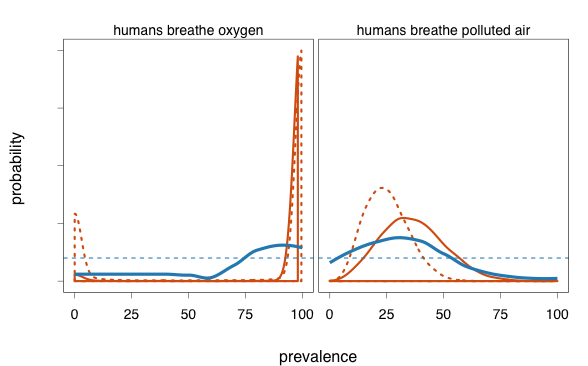
\includegraphics[width=0.7\columnwidth]{example}
%    \caption{Different priors on prevalence lead to dramatically different interpretations of the generic. Orange: prevalence. Blue: threshold for the generic to be true. Dotted lines denote priors and solid lines denote posteriors. Breathing oxygen is something that almost every animal-kind does (and within each kind, 100\% of them do). Breathing polluted air is a more accidental condition, and animal kinds will differ in how many of them are exposed to polluted air.}
%  \label{fig:ex}
%\end{figure}
%
%
%Consider again the case of vague adjectives. \emph{Tall} means something different if it is predicating ``John'' than if it is predicating ``The Empire State Building'' because the distributions over heights vary for people and buildings. In the people domain, $\theta_{tall}$ will probably be set somewhere around 6 feet, since this is above the mean (and hence, would be informative) but not too far above the mean (hence, would still be truthful). 

%\subsection{The \emph{Question Under Discussion}}
%
%To connect this model to the dependent measures used in the experiments that follow, we introduce another level to the model. One of the tasks is a true-false judgment task, which we model as a speaker who can either say ``[[the generic]] is true'' or ``[[the generic]] is false''.
%
%\begin{equation} 
%P_{S_{2}}(g \mid x) \propto {P_{L_{1}}(x \mid g)}.
%\label{eq:S2}
%\end{equation}
%
%This speaker in \eqref{eq:S2}, like $L_{1}$, doesn't know the threshold, but knows that $L_{1}$ is thinking about it, and marginalizes over possible values: $ P_{L_{1}}(x \mid g) = \sum_{\theta} P_{L_{1}}(x , \theta \mid g) $.
%
%In the other task, participants are given a generic utterance and asked to judge the prevalence of the property. 
%



%As a first test the model, we posit a family of possible priors $x \thicksim \beta(\gamma,\delta)$\footnote{For ease of interpretation, we are parametrizing the $\beta$ distribution by its mean and concentration. To recover the canonical shape parametrization, use $\gamma \delta$ and $(1-\gamma)\delta$.}. We hypothesize that the details of these priors (i.e.~$\gamma$'s and $\delta$'s) may differ according to the type of property in reference by the generic. For instance, when you know that a particular property is rare, a different distribution of that property over kinds is called to mind, than if the property is common. This would result in different meanings for the generic. Below we infer appropriate prior parameters for each property-type from the behavioral data.
%
%Following the advice of \citeA{Degen2014}, who investigated the relationship between dependent measures and speaker and listener roles in RSA, we will model the \emph{implied prevalence} task as a pragmatic listener ($L_{1}$) task, but the \emph{truth conditions} task as a pragmatic speaker task. We model the truth judgment with a speaker $S_{2}$ who is trying to convey the prevalence to a pragmatic listener, but can only produce the generic or its negation (i.e.~yes or no to the truth of the generic):

\section{Experiment 1: Truth value judgments}

The lifted-threshold RSA model specified in Eq.~\ref{eq:S2} predicts probabilities of producing a generic given a prior distribution on the prevalence of the property. 
In Expt.~1a, we measure the distribution on prevalence of certain target properties by asking participants about the percentage of a kind with the property \footnote{So as to not bias the measurement in favor of a small number of stipulated animal categories, we ask participants to generate their own animal categories.}. 
In Expt.~1b, we measure the acceptability of a number of generic statements about the properties measured in Expt. 1a. 
We show how the prevalence within a property alone is insufficient to explain the diversity of truth judgments of these generics, but how a model of a pragmatic speaker who considers the distribution on prevalence can explain this wide range of truth judgments.

\subsection{Experiment 1a: \emph{Eliciting the prior}}

The goal of this experiment was to measure participants' beliefs about the distributions of the prevalence of various properties within and across categories.

\subsubsection{Participants}

We recruited 30 participants over Amazon's crowd-sourcing platform Mechanical Turk (MTurk).  Participants were restricted to those with US IP addresses and with at least a 95\% MTurk work approval rating. All participants were native English speakers. The experiment took about 10 minutes and participants were compensated \$1.00.

\subsubsection{Procedure and materials}

On each trial of the experiment, the participant filled out a table where each row was an animal category and each column was a property\footnote{The experiment in full can be viewed at \url{http://stanford.edu/~mtessler/experiments/generics/experiments/real-kinds/prior-2.html}}. 
Participants were asked to respond with the percentage of the species that had the property.
The list of animal categories was only partially pre-specified with animal categories that would be used in the generic truth judgment task.
%These names were randomly sampled from a larger set of categories of interest (see Appendix \ref{sec:appendix} for full list of animals and properties used). 
Participants were asked to add five of their own animal names to the list. 
Upon completion, the next column appeared with a property (e.g. ``has manes'') as the column header and text-boxes where the participants could put their estimated prevalence. 
%Participants were asked: ``For each kind of animal, what percentage of the species do you think [property]?'' 
This procedure was repeated for 8 properties in total. 
The animal kind column was unable to be modified once completed. 
The prevalence columns, however, could be modified at a later stage (i.e. the participant could go back and change her estimates after seeing more properties). 
Participants completed this procedure on each of 2 trials.

We used a set of properties associated with generics of theoretical interest (16 properties in total), motivated in part by conceptual distinctions pointed out by \citeA{Prasada2013}. 
The conceptual categories used to generate the generics were: majority characteristic (e.g. ``Leopards have spots''), minority characteristic (e.g. ``Lions have manes''), striking (e.g. ``Sharks attack swimmers.''), and majority false generalizations (e.g. ``Ducks are female.'') \cite{Prasada2013}. In addition, we included false sentences (e..g ``Lions lay eggs''), to cover the full range of possible truth values .
%The pre-specified animal names were those names associated with these generics.  
For a full list of the generic sentences used in this experiment, see Appendix \ref{sec:appendix}.
Complete instructions given to participants can be seen in Appendix \ref{sec:prior1instruct}.



\subsubsection{Bayesian data analysis}
\label{sec:bda1}

There is important latent structure in the prior elicitation task. 
Responses $d$ can be categorized into those that reflect the property is present in the species or absent in the species. 
If the property is absent, then the response is 0\% of the species has the property. 
The number of 0 responses act as an indicator of the prevalence of the property \emph{across categories} $\theta_{across}$ (for example, ``are female'' would have very few 0\% responses, whereas ``have feathers'' would receive appreciably more, owing to the fact the prevalence of these properties \emph{across categories} is different).

\begin{align*}
d_{across} & \sim \text{Bernoulli}(\theta_{across}) \\
d_{across} & = \begin{cases}
				1 & \mbox{if } d > 0 \\
				0 & \mbox{if } d = 0 
				\end{cases}
\end{align*}

For those responses that reflect the property is present ($d > 0$), assume those responses come from a distribution with some mean and variance ($\gamma_{within}, \gamma_{across}$), and try to infer that distribution. 
Since the responses vary between 0 - 100, the natural distribution is a Beta distribution. 

$$
d_{across} \sim \text{Beta}(\gamma_{within}, \gamma_{across})   \mbox{ if } d > 0
$$

We implemented this Bayesian statistical model using the probabilisitic programming language WebPPL \cite{dippl}. We used the Metropolis-Hastings algorithm to estimate the posterior distribution over the latent parameters $\theta_{across}, \gamma_{within}, \delta_{within}$ with X chains of Y samples.

To reconstruct the likely distribution of  prevalence both within- and across- categories, we took samples from the posterior predictive distribution of $d$ by running the forward model: 

\begin{align*}
h & \sim \text{Bernoulli}(\theta_{across}) \\
x & \sim \begin{cases} 
		\text{Beta}(\gamma_{within}, \delta_{within}) &\mbox{if } h = 1 \\ 
				0 & \mbox{if } h=0
				\end{cases} 
\end{align*}

where, $h$ is a variable indicating whether or not the property is present within a particular species. 


We also inferred the likely prevalence of each animal category and property pair of interest, to be used in the generic truth judgment task (Expt.~1b). The results of this can be seen in Table \ref{tab:expt1}.

%\begin{align*}
%d_{across} \sim \text{Beta}(\gamma_{across}, \delta_{across}) \\
%d_{within} \sim \text{Beta}(\gamma_{within}, \delta_{within}) 
%\end{align*}
%The parameters $\gamma$ and $\delta$ correspond to the mean and variance (formally, the concentration), respectively, of prevalence for each of the across- and within- distributions. 
%We put identical, uninformative priors on these parameters:
%\begin{align*}
%\gamma & \sim \text{Uniform}(0,1) \\
%\delta & \sim \text{Uniform}(0,10)
%\end{align*}
%To construct single prevalence distributions reflecting both the within- and across- category prevalence (as we have for Expt.~1a), we assume that the distribution is a mixture of categories that have the property and categories that don't have the property\footnote{This is similar in spirit to Hurdle Models of count data used in clinical trials where the observed proportion of zeros is greater than one would expect from classical models of count data like the Poisson model.}. Whether or not a category has a property is determined by flipping a coin, weighted by the prevalence across categories
%\begin{align*}
%\theta_{across} & \sim \text{Beta}(\gamma_{across}, \delta_{across}) \\ 
%h & \sim \text{Bernoulli}(\theta_{across}) \\
%x & \sim \begin{cases} 
%		\text{Beta}(\gamma_{within}, \delta_{within}) &\mbox{if } h = 1 \\ 
%				0 & \mbox{if } h=0. 
%				\end{cases} 
%\end{align*}

\subsubsection{Results}

We expected the prevalence priors to be qualitatively different for the different properties. 
Each participant gave responses to the 12 animal categories that were fixed as well as to 10 animal categories that the participant herself produced. 

From the 300 free responses for the animal production part of the task, 105 distinct animal names were extracted. The top 5 ranking animal names produced were Dog, Cat, Elephant, Giraffe, and Bear; these responses accounted for 20.3\% percent of the total produced animal names.

\begin{figure}
\centering
    \includegraphics[width=0.8\columnwidth]{prevalence_priors_inferred-gammas.pdf}
    \caption{Four example elicited prevalence priors inferred using a Bayesian statistical model. 
    Density plots reveal qualitatively different distributions for different properties. 
    Each sample from these distributions can be thought of to correspond to a particular animal category, representing the prevalence of the property within that animal category.}
  \label{fig:priors1a}
\end{figure}

%We aggregated responses for each property by rounding responses to the nearest 10 and constructing a histogram. 

We analyzed responses for each property using the Bayesian data analytic approach described in Section \ref{sec:bda1}.	
The most likely prevalence priors inferred from the data are shown in Figure \ref{fig:priors1a} for 4 example properties.
We observe substantial differences between the priors over prevalence. 
In accord with intuition, the property ``is male'' is highly prevalent across categories, but within a category is only present in about 50\% of cases.
By contrast, ``has manes'' is rare across categories, but has the same prevalence within-categories as ``is male'', reflected by the bump in density around 50\% (Figure \ref{fig:priors1a} bottom left).
The property ``has wings'' is also relatively rare across categories, but within a category is widespread, as reflected by the bimodal distribution. 
Finally, ``has malaria'' is an example of a property that is both rare across-species and within-species. 
The property is absent from most animal species, and even when it is present, it is only present in a small number of cases.


%There are fewer responses for some animal categories relative to others, owing to idiosyncratic differences in the availability during the production part of the experiment (e.g. ``Dog'' is produced 10 times more than ``Bee'') as well as the fact that our 12 target categories were presented to every participant (whereas the freely-produced categories were not). 
%As a result, these distributions may be biased to over-represent certain animal categories. 
%However, the distributions produced by analyzing the data on a by-response or by-category were qualitatively similar. 
%In addition, model predictions between the the model using the by-response prior distribution and the by-category distribution had a correlation of \red{r = X.XX}, suggesting that the variability that is leads to different rates of generic acceptability were captured by the shared variance of these distributions. 


\subsection{Experiment 1b: \emph{Truth judgments of natural cases}}

The goal of this experiment was to measure participants' beliefs about the acceptability of a number of different generic sentences. 


\subsubsection{Participants}

We recruited 100 participants over Amazon's crowd-sourcing platform Mechanical Turk (MTurk).  Participants were restricted to those with US IP addresses and with at least a 95\% MTurk work approval rating. All participants were native English speakers. The experiment took about 3 minutes and participants were compensated \$0.35.

\subsubsection{Procedure and materials}

We used a two-alternative forced-choice (2AFC) paradigm to measure participants' beliefs about the acceptability of 30 generic sentences. 
Data reported in \citeA{Prasada2013} revealed that participants assign midpoint ratings on a Likert scale to anomalous generics like ``Birds are female''. 
We hypothesized that these ``neither true nor false'' ratings would be translated into more graded responses across the population using the 2AFC (i.e. subjects would be closer to chance).

Participants were asked to report whether they agreed or disagreed with generic sentences presented in bare plural form (e.g. ``Birds lay eggs.''). 
Items were presented sequentially, and subjects reported whether or not they agreed with the sentence by pressing either ``P'' or ``Q'' (randomized between-subjects). 
Generic sentences were selected to correspond with the prevalence distributions elicited in Experiment 1a. 
Approximately 10 true, 10 false, and 10 uncertain truth-value generics were selected (see Appendix \ref{sec:appendix} for full list of items).
As a manipulation check, participants were asked at the end of the trials which button corresponded to ``Agree''.

\subsubsection{Results}

Four participants were excluded for failing to successfully report which button corresponded with ``Agree''. 
Five additional participants were excluded for listing a language other than English as their native language, resulting in 91 participants.


\begin{figure}
\centering
    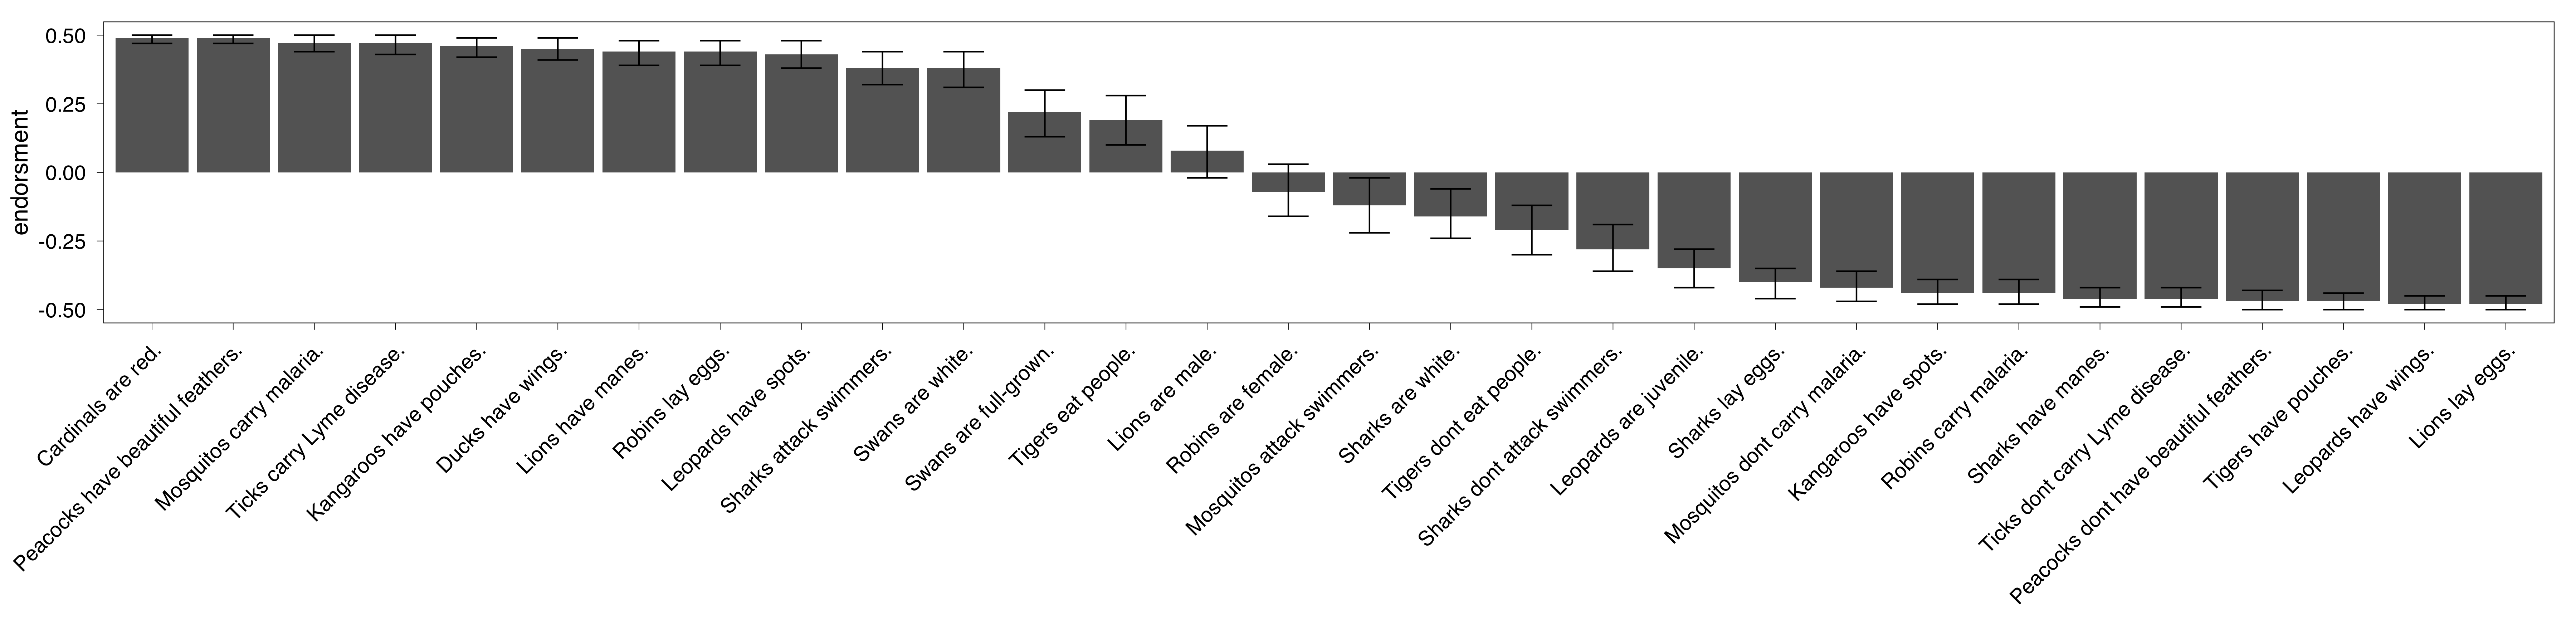
\includegraphics[width=\columnwidth]{truhtjudge_n100}
    \caption{Truth judgments from Expt.~1b for each item. Y-axis denotes deviations from chance in the 2AFC. There is large agreement for both generics which are true and generics which are false. There is considerable disagreement across participants for a number of ``neither true nor false'' generic statements. }
  \label{fig:tj1b}
\end{figure}


The 30 generic sentences fell into 3 \emph{a priori} categories: definitely true, definitely false, and neither true nor false (Figure \ref{fig:tj1b}). We entered participants' agreement judgments into a mixed-effect logistic regression with random by-participant effects of intercept. 
This \emph{a priori} distinction was a significant predictor of the eventual truth judgments: true generics were significantly more likely to be agreed with than the indeterminate generics ($\beta = 3.14; SE = 0.15; z = -20.9$).
Indeterminate generics were agreed with \emph{less} likely than chance ($\beta = -0.49; SE = 0.09; z = -5.3$) but significantly more than false generics ($\beta = 2.07; SE = 0.15; z = 14.1$).

Truth judgments for these generic sentences were correlated with the prevalence of the property for the target category elicited in Expt.~1a ($r = 0.73$, Figure \ref{fig:scatterprev}). This is, of course, expected given that high-prevalence true generics (e.g. ``Leopards have spots.'') and low-prevalence false generics (e.g. ``Leopards have wings.'') were used. 
However, large deviations from a purely within-category prevalence account remain: Generics with intermediate prevalences (Prevalence quartiles 2 and 3: $ 22\% < prevalence < 62\%$), exhibited no correlation with truth judgments ($r_{Q2,3} = -0.08$).


\begin{figure}
\centering
    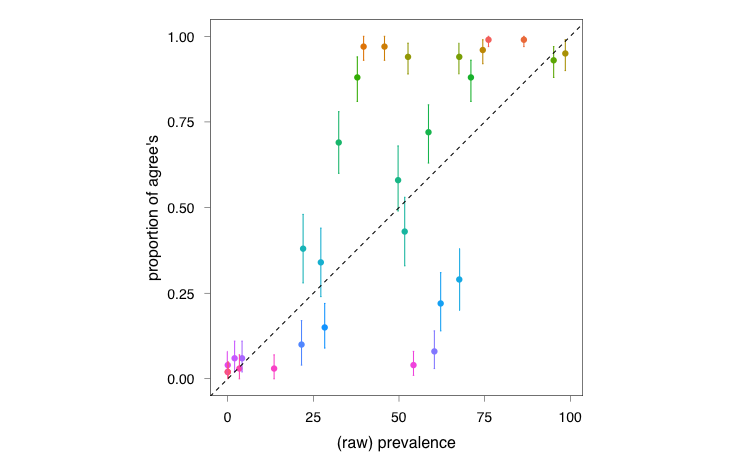
\includegraphics[width=0.8\columnwidth]{tj_n50_tjVsPrevalence}
    \caption{Truth judgments from Expt.~1b for each item vs. the prevalence of the property for the target item as measured in Expt.~1a. For example, ``Leopards have spots'' has a very high truth judgment (Expt.~1b; Y-axis), and ``has spots'' is a highly prevalent property for leopards (Expt.~1a; X-axis). Color spectrum corresponds to the rank ordering of the truth judgment data; similarly colored dots received similar truth judgments.}
  \label{fig:scatterprev}
\end{figure}




\subsection{Lifted-threshold model predictions}

The model specified in Section \ref{sec:model} reasons about the likely prevalence that a listener will infer given an informative speaker, a generic sentence and a distribution over the prevalence of the property. 
In this way, the model takes into account the prevalence of the property both within- and across-categories.
We explore the predictions of this model, using the empirical priors elicited in Expt.~1a. 
We compare these predictions to the truth judgment data observed in Expt.~1b.

\subsubsection{Posterior over model parameter}

The model has one free parameter, the speaker rationality in Equation \ref{eq:S1}. 
We also explicitly model guessing behavior as a source of contamination of the observed data. This is done by positing the data generating process is a mixture of random guessing and pragmatic reasoning. We put uncertainty over the mixture parameter $\phi$, which represents the proportion of the data that can be better explained by random guessing than by our model of pragmatic reasoning.
In this way, $\phi$ provides a crude measure of goodness of fit. 
We put a uniform prior over this variable and infer its credible values using a Bayesian statistical model. 

To learn about the \emph{a posteriori} credible values of our model parameter, we used the probabilistic programming language WebPPL \cite{dippl} to collect \red{X} chains of \red{Y} samples using the Metropolis-Hastings algorithm. 
The estimated posterior density of this parameter is shown in Figure \ref{fig:rationality}. 
This parameter represents the speaker's belief in how rational the hypothetical listener believes he is when choosing to say the generic (over saying nothing). 
The 95\% Credible Interval is [3.79,4.70].

\begin{figure}
\centering
    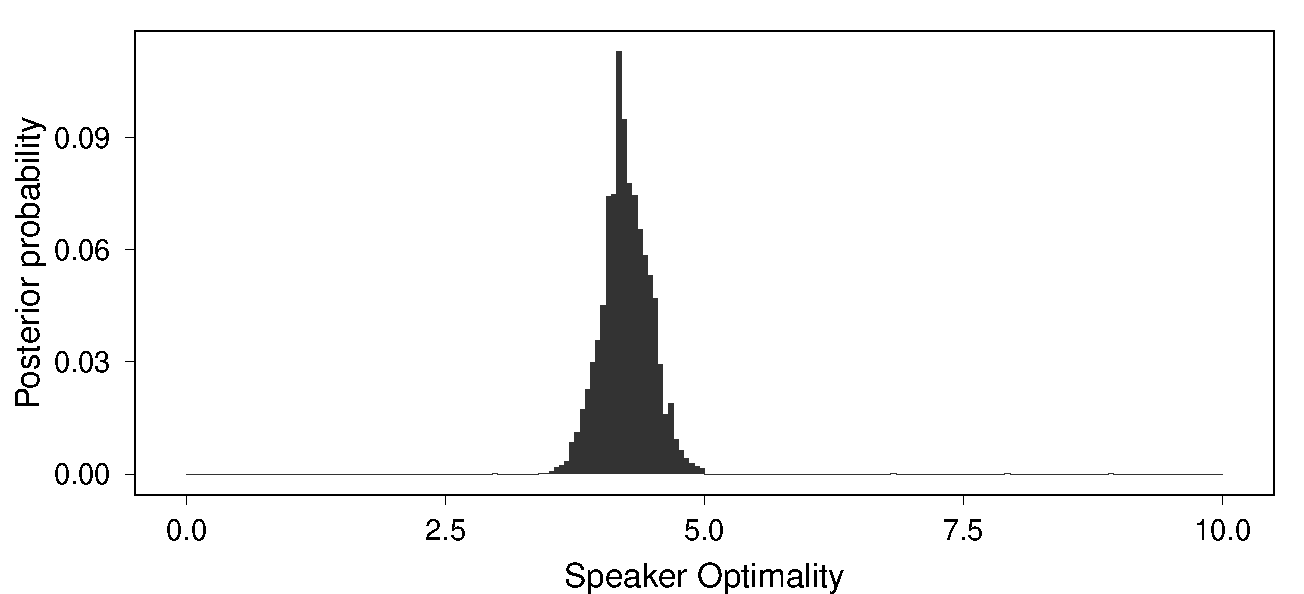
\includegraphics[width=0.8\columnwidth]{posterior-rationality-truthJudge}
    \caption{Posterior distribution of the speaker rationality parameter.}
  \label{fig:rationality}
\end{figure}


\subsubsection{Posterior predictive}

We evaluate the model by examining the posterior predictive distribution of responses. The posterior predictive distribution marginalizes over the inferred parameter values to produce predictions about what the data should look like given the lifted-threshold model and the observed data. This is akin to fitting the parameters and is an important step in model validation: It shows what data is actually predicted by the model. 
Figure \ref{fig:modeldataScatter} shows the expected values of the model predictions compared against the observed data. 
The model predicts graded endorsements for the generic statements used in Expt.~1b. 

\begin{figure}
\centering
    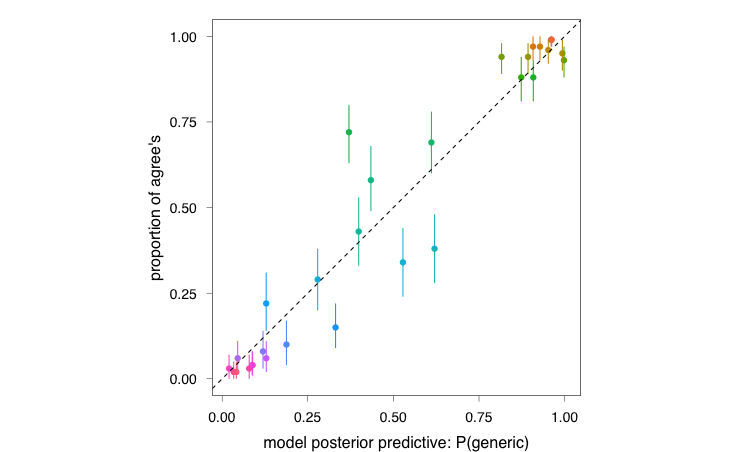
\includegraphics[width=0.8\columnwidth]{tj_n100_tjVsPostpred}
    \caption{Truth judgments from Expt.~1b for each item vs. the posterior predictive expected value for the target item using the lifted-threshold model with the empirical priors elicited in Expt.~1a. Color spectrum corresponds to the rank ordering of the truth judgment data; similarly colored dots received similar truth judgments.}
  \label{fig:modeldataScatter}
\end{figure}

The model captures the data well ($r=0.96$). 
Generics that received definitive agreement or disagreement are predicted to be judged as such by the model (corners of Figure \ref{fig:modeldataScatter}). Unlike the model based on within-category prevalence alone, the lifted-threshold model does not break down for generics of categories with intermediate prevalence of the property; for $ 25\% < prevalence < 75\%$, the correlation is $r=0.94$. Indeed, the model captures the rank ordering of the truth judgments of these generics well ($r_{spearman} = 0.94$); the color gradient in Figure \ref{fig:modeldataScatter} is smooth, unlike what is observed when comparing the data against within-category prevalence alone (Figure \ref{fig:scatterprev}). 

The largest deviations occur for the items with greatest variance (``neither true nor false'' generics). For example, ``Mosquitos attack swimmers'' was predicted to be a relatively good generic (expected value of model predictions: 0.62; observed proportion agreement: 0.38). This is because in Expt.~1a, participants estimated that on average approximately 20\% of mosquitos attack swimmers. This high prevalence (relative to the empirical distribution), produced this strong prediction. It's possible that the truth judgment task called to mind salient alternatives like ``Mosquitos bite swimmers'' whereas the prior elicitation task did not. Another item with large deviation is ``Swans are full-grown'' (expected value of model predictions: 0.37; observed proportion agreement: 0.70). Again, this may be due to uncertainty of the participants about whether or not there is a label for juvenile swans (akin to ``pups'' for ``dogs''). We return to this sort of uncertainty in the general discussion.


\subsection{Discussion}

In Expt.~1, we asked whether or not participants' truth judgments on a set of generic sentences covering a range of conceptual distinctions could be explained by a language understanding model with a truth-functional threshold sensitive to the prior distribution over prevalence. 
In Expt.~1a, we empirically measured the prior distribution of prevalence by asking participants about their beliefs of how prevalent certain properties are across many animal categories. 
Here, we observed qualitatively different distributions corresponding to properties that are common within-categories and common across-categories (e.g. ``are male''), common within-categories but rare across-categories (e.g. ``have manes''), rare within-categories and rare across-categories (e.g. ``carries malaria''). Interestingly, these same distinctions are made between generics of these properties \cite{Prasada2013}. 
Our empirical and modeling results suggest these distinctions are a result of different belief distributions about the prevalence of the properties.

How does the model arrive at different truth judgments for generics of different properites?
Here, the prevalence prior plays a critical role in determining where the generic-threshold $\theta$ (and, consequently, the resulting inferred prevalence $x$) is likely to fall (see Figure \ref{fig:priors1a} for examples of the relevant priors). 
In setting the threshold, the pragmatic listener $L_{1}$ balances the truth of the utterance with the informativeness of the utterance. 
If the pragmatic listener hears ``Lions haves manes.'', she will likely set the threshold $\theta$ below 50\%, as this is necessary to make the utterance true (Figure \ref{fig:priors1a} bottom left). 
At the same time, the listener believes the message to be informative, so she will probably set $\theta$ above 10\%. 
Since the posterior inferred prevalence has to be greater than the threshold in order to make the utterance true, the most likely inferred prevalence $x$ will be about 50\% (i.e. after ruling out everything below 10\%, the most probably prevalence will be 50\%). 
Since this matches the speaker's believed prevalence of having manes among lions, the speaker concludes the generic is a helpful thing to say.
%These differences, coupled with a vague meaning for the generic, produce different acceptance probabilities for a range of generic sentences. 
%For example, ``Mosquitos carry malaria'' is true, because the prevalence of malaria among mosquitos is higher than prevalence of malaria among most (possibly all) other animal species. 
%``Lions have manes'' is true for the same reason. 
At the same time, participants judged ``Lions are male'' to be neither true nor false; the model exhibits the same behavior because the prevalence of being male among lions is neither significantly more nor less than prevalence of being male among other animal species. 

The conceptual distinctions among generics \cite{Prasada2013} explored in this experiment can be explained by differences in the distribution of the prevalence of these properties. 
Our model of a speaker considering a listener who has uncertainty about the true threshold on prevalence produces truth judgments highly similar to those of our participants.

%The speaker selects the utterance according to a soft-max decision rule governed by parameter $\lambda$\footnote{It's conceivable that this $\lambda$ is different from the parameter that governs the selection of $S_{1}$'s utterances. For simplicity here we assume they are the same.}.


%To connect our model of generic interpretation to generic truth conditions, we include an additional component to the model: a speaker who can either say ``[[the generic]] is true'' or ``[[the generic]] is false'' \cite{Degen2014}:

%\begin{equation} 
%P_{S_{2}}(g \mid x) \propto \exp(\lambda \ln {P_{L_{1}}(x \mid g)}).
%\label{eq:S2}
%\end{equation}
%
%
%This speaker in \eqref{eq:S2}, like $L_{1}$, doesn't know the threshold, but knows that $L_{1}$ is thinking about it, and marginalizes over possible values: $ P_{L_{1}}(x \mid g) = \sum_{\theta} P_{L_{1}}(x , \theta \mid g) $. The $S_{2}$ speaker has in mind a prevalence $x$ (or, equivalently here, a category--property pair corresponding to that prevalence), e.g. ``birds'' and those that ``lay eggs''. The speaker then reasons whether it would be better to say ```Birds lay eggs' is true''  or ```Birds lay eggs' is false'' in order to convey the state of the world, namely that about 50\% of birds lay eggs\footnote{Technically, the prevalence of birds laying eggs is closer to 35\%, as only \emph{adult}, female birds lay eggs. We gloss over this detail here.}. The speaker selects the utterance according to a soft-max decision rule governed by parameter $\lambda$\footnote{It's conceivable that this $\lambda$ is different from the parameter that governs the selection of $S_{1}$'s utterances. For simplicity here we assume they are the same.}.
%
%Continuing with this example, the speaker imagines the likely prevalence that the pragmatic listener $L_{1}$ will infer given either ```Birds lay eggs' is true''  or ```Birds lay eggs' is false''. Here, the prevalence prior plays a critical role in determining where the generic-threshold $\theta$ (and, consequently, the resulting inferred prevalence $x$) is likely to fall (Figure \ref{fig:schematic}). In setting the threshold, the pragmatic listener $L_{1}$ balances the truth of the utterance with the informativeness of the utterance. If ```Birds lay eggs' is true'', the pragmatic listener $L_{1}$ will likely set the threshold $\theta$ below 50\%, as this is necessary to make the utterance true (Figure \ref{fig:schematic}; red). At the same time, $L_{1}$ believes the message to be informative, so she will set $\theta$ probably above 10\%. Since the prevalence has to be above the threshold in order to make the utterance true, the most likely inferred prevalence $x$ will be about 50\% (i.e. after ruling out everything below 10\%, the most probably prevalence will be 50\%). On the other hand, if the speaker were to say ```Birds lay eggs' is false'', the prevalence would have to fall \emph{below} the threshold, which in this case would implicate the mass below 10\% and the pragmatic listener would infer something the speaker didn't intend. 


\section{Experiment 2: Generics carry strong implications}

Generic statements are endorsed for a seemingly puzzlingly wide range of prevalence levels. 
However, this puzzle is resolved when a speaker understands the generic to be vague and takes into account the distribution of the property in question within- and across- categories. 
A second puzzle surrounds how a listener is to interpret a generic utterances.
Some of the earliest psychological work on generics brought this out, suggesting that generics ``once accepted psychologically, ... appear to be commonly taken in a rather strong sense, as if the qualifier \emph{always} had implicitly crept into their interpretation'' \cite{Abelson1966}. \red{[Note: this is the same quote that Cimpian2010 use... is this okay?}.
%
\citeA{Gelman2002} found that adults interpret novel generic statements about familiar kinds (e.g. ``Bears like to eat ants.'') as implying that almost all of the category has the property (e.g. almost all bears like to eat ants).
\citeA{Cimpian2010} found similar inferences with generics about unfamiliar kinds (e.g. ``Lorches have purple feathers.''). 

These strong inferences are puzzling when examined next to the prevalence required for a generic to be true. 
As we saw in Expt.~1, generics can be true for a range of prevalence levels. 
This phenomenon clearly distinguishes generic statements from quantified statements.
``All lorches have purple feathers.'' is true only when 100\% of lorches have purple feathers. 
Similarly, upon hearing such an utterance, one is likely to infer that 100\% of lorches have purple feathers.  
This symmetric relationship was found to hold with the quantifier ``most'', but generic utterances don't behave in this way \cite{Cimpian2010}.
%Participants judged ``most'' sentences true when between 50-100\% of the category had the property (on average: 75\%). 
%Similarly, upon hearing an utterance with ``most'', participants on average inferred a prevalence of about 75\%. 
Generic statements are judged true for a wide range of prevalence levels, but upon hearing a generic utterance, participants were wont to infer that \emph{all} or \emph{almost all} of the category have the property. 
Thus, the implications of generic statements go far beyond the evidence needed to accept them as valid.

Not all statements in bare plural form carry these implications, however. 
Indeed, interpretations of these sentences are sensitive to listener's beliefs about the properties in question. 
\citeA{Cimpian2010} observed that predicating with accidental properties (e.g. ``Lorches have muddy feathers.'') significantly reduced participants' judgments about the implied prevalence of these statements.

%That is, when the property in question was dangerous and distinct, participants required a lower overall prevalence (e.g. 10\% of lorches had purple feathers) to assert that the generic statement was true.

Expt.~2 attempted to replicate, extend and explain the findings of \citeA{Cimpian2010}: that there is an asymmetry between truth conditions and implied prevalence of the generic and that this asymmetry is sensitive to the type of property predicated. 
In Expt.~2a, we measure participants' beliefs about the distribution of these types of properties using a paradigm generalized from Expt.~1a. 
In Expt.~2b, we replicate and extend \citeauthor{Cimpian2010}'s findings to different classes of properties for which the prevalence priors differed. 
We show that the language understanding model predicts this asymmetry between truth conditions and implications, and that this asymmetry can be manipulated by differences in the prevalence distributions between properties.

%Exp. 1a and 1b were conducted on separate sessions, one week apart. None of the participants completed both experiments.


\subsection{Experiment 2a: \emph{Prior elicitation for properties of novel animals}}

In this experiment, we measured participants' beliefs about the distribution of the prevalence of a certain property within- and across- animal kinds. 
We used materials from \citeA{Cimpian2010} which consisted of novel animal categories (e.g. glippets) and various properties (e.g. have orange legs; have broken legs).


\subsubsection{Participants}

We recruited 40 participants over Amazon's crowd-sourcing platform Mechanical Turk (MTurk).  Participants were restricted to those with US IP addresses and with at least a 95\% MTurk work approval rating. All participants were native English speakers. The experiment took about 5-7 minutes and participants were compensated \$0.75.

\subsubsection{Procedure and materials}

In Expt.~1a, participants filled out a table with rows corresponding to different animal kinds and columns corresponding to different properties. 
Pilot testing suggested this was a pragmatically strange setup for this paradigm: answering ``What percentage of lorches have purple feathers?'', when participants knew nothing about lorches was difficult.
We thus generalized the procedure to ask simpler questions and used a Bayesian statistical model to infer the underlying distribution. 
We then used these distributions in our language model to make predictions about the implications of generic sentences.

Participants were asked about the prevalence across categories by asking them the likelihood of there existing a K that has F, where K was a novel animal categories and F was a property (e.g. ``how likely is it that there is a lorch that is female?''). 
Prevalence within categories was measured by asking participants about the percentage of Ks that have Fs, given that at least one does.
Complete instructions shown to participants are in Appendix \ref{sec:prior2instruct}. 

Participants responded using slider bars that ranged from ``unlikely'' to ``likely'', and ``0\%'' to ``100\%'', respectively.

Materials---novel animal names and familiar properties---built upon those from \citeA{Cimpian2010}. 
Classic work in generalization suggested to us that there may be differences in the distributions of different types of biological properties \cite{Nisbett1983}. 
We expanded the stimulus set to include four different types of properties: biological parts (e.g. ``feathers''), colored parts (e.g. ``purple feathers''), vague parts (e.g. ``smooth feathers''), and accidental parts (e.g. ``broken feathers''). 
Pilot testing revealed a lot of variability in the estimated prevalences of accidental properties relative to the other types of properties. 
To test the quantitative predictive power of the generic interpretation model, we used twice as many exemplars of the accidental class of properties, with the aim to make a ``common accidental'' and a ``rare accidental'' class of properties. 
We used 8 exemplars of each of the three non-accidental properties (``parts'', ``colored parts'', ``vague parts'') and 16 exemplars of accidental properties.
Materials are in Appendix \ref{sec:materials2}.

\subsubsection{Data analysis}

In order to recover single belief distributions representing prevalence both within- and across- categories (analogous to those elicited in Expt.~1a and shown in Figure \ref{fig:priors1a}), we built a simple Bayesian statistical model of the task questions and their relation to the desired distribution. 

Participants' responses to each question (slider bar values) were assumed to be samples from Beta distributions with unknown parameters. 
The responses to the questions ($d_{across}, d_{within}$) were used to estimate the parameters of the distributions of prevalence across- and within- categories, separately. 
\begin{align*}
d_{across} \sim \text{Beta}(\gamma_{across}, \delta_{across}) \\
d_{within} \sim \text{Beta}(\gamma_{within}, \delta_{within}) 
\end{align*}
The parameters $\gamma$ and $\delta$ correspond to the mean and variance (formally, the concentration), respectively, of prevalence for each of the across- and within- distributions. 
We put identical, uninformative priors on these parameters:
\begin{align*}
\gamma & \sim \text{Uniform}(0,1) \\
\delta & \sim \text{Uniform}(0,10)
\end{align*}
To construct single prevalence distributions reflecting both the within- and across- category prevalence (as we have for Expt.~1a), we assume that the distribution is a mixture of categories that have the property and categories that don't have the property\footnote{This is similar in spirit to Hurdle Models of count data used in clinical trials where the observed proportion of zeros is greater than one would expect from classical models of count data like the Poisson model.}. Whether or not a category has a property is determined by flipping a coin, weighted by the prevalence across categories
\begin{align*}
\theta_{across} & \sim \text{Beta}(\gamma_{across}, \delta_{across}) \\ 
h & \sim \text{Bernoulli}(\theta_{across}) \\
x & \sim \begin{cases} 
		\text{Beta}(\gamma_{within}, \delta_{within}) &\mbox{if } h = 1 \\ 
				0 & \mbox{if } h=0. 
				\end{cases} 
\end{align*}

Marginal posterior distributions for $x$ for estimated using the Metropolis-Hastings algorithm in the probabilistic programming language WebPPL \cite{dippl}. Inference was completed by taking 50,000 samples using the Metropolis-Hastings algorithm.

\subsubsection{Results}

Our focus for this experiment is to see if the distributions on prevalence differ between the different types of properties.
We analyzed the data first by item in order to split the accidental properties into two categories: common accidental properties (e.g. wet fur) and rare accidental properties (e.g. broken legs). We then ran the model again analyzing the data by type of property.

Figure \ref{fig:prior2} Left shows the posterior predictive distributions for prevalence $x$ for 5 different types of properties.Figure \ref{fig:prior2} Right shows the region of interest of these distributions by removing the all the mass at 0. These distributions form the prevalence priors used in the language understanding model. 
With the exception of the body part category, properties are mostly likely to be absent from the category (Figure \ref{fig:prior2} left; modes of distributions are at 0).
If the property is present in the category, the most likely prevalence for biological properties (``part'', ``color part'', and ``vague part'') is 100\% (Figure \ref{fig:prior2} right; modes of blue, green, and red distributions are at 1).
This is not the case with the prevalence priors for accidental properties, for which lower values are more likely (Figure \ref{fig:prior2} right; modes of orange and purples distributions are at some low prevalence).


\begin{figure}
\centering
    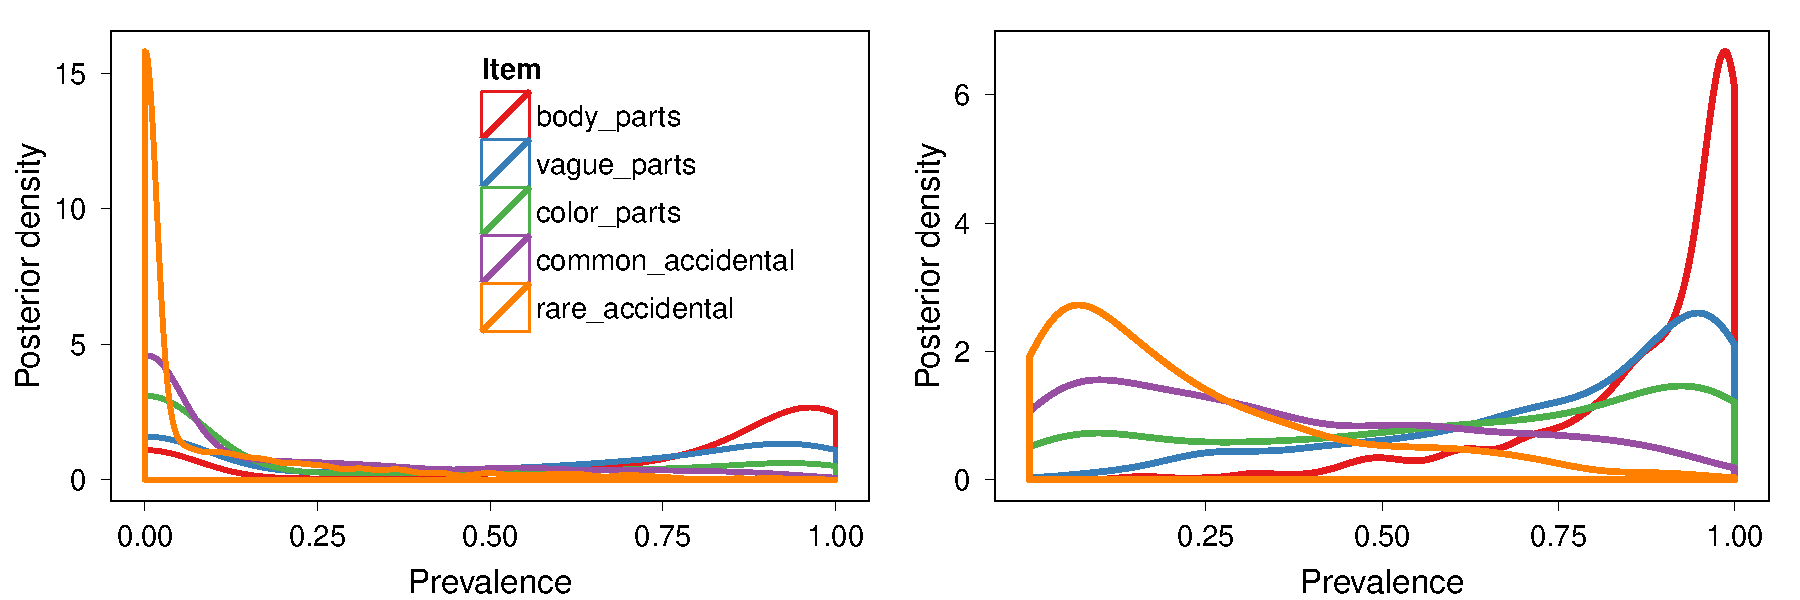
\includegraphics[width=\columnwidth]{prior2_prevalenceprior-50k.pdf}
    \caption{Prevalence priors inferred from the prior elicitation experiment  (Expt.~1a). Right plot shows all non-zero probability mass. This corresponds to the expected within-category prevalence. Different types of properties have different likely prevalence values.}
  \label{fig:prior2}
\end{figure}

%
%In Section \ref{sec:model1}, we posited a family of priors for our model (the $\beta$ family of distributions). We saw that our model could accommodate both the flexibility in truth conditions as well as the asymmetry between truth conditions and implications. This combined data-analysis --- cognitive model made the \emph{backward prediction} that the priors would have to vary between property-types. In Exp.~2 we found that to be case \footnote{Qualitative differences between the \emph{observed} and \emph{backward-predicted} priors are likely a results of the family of priors posited a priori. The $\beta$ family can only accommodate U- and N- shaped distributions.}. There is still a question of whether or not the priors elicited in Exp.~2 would actually still predict the flexible truth conditions and the asymmetry.  
%
%To test this, we fix the rationality parameters $\lambda_{task}$ as the fit-value to be the Maximum A-Posteriori (MAP) values from the Bayesian model analysis above. We then sample, with replacement, subjects from our prior elicitation task in order to bootstrap our model predictions. The confidence intervals thus reflect the uncertainty in our model predictions attributable to uncertainty in the empirical prior data\footnote{The model predictions are generated using exact enumeration, so there uncertainty in the model predictions due to posterior sampling error.}. 
%
%
%
%Figure \ref{fig:exp1preds} shows the model predictions for the truth conditions using the empirical prior data from Expt. 2. Like the model with $\beta$ family hyperpriors, the empirical prior model captures the flexibility in truth conditions across the three property types. Figure \ref{fig:model_asyms} shows the predicted ``strong implications'' for the biological type properties used in Expt. 1.


%\begin{figure}
%\centering
%    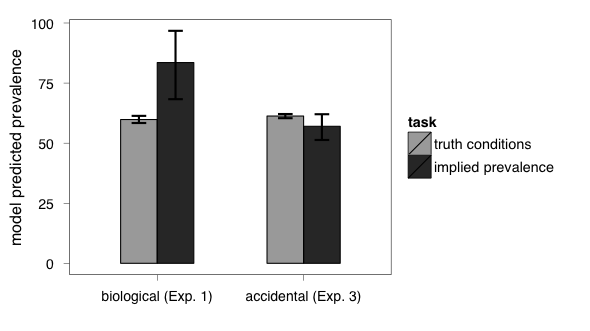
\includegraphics[width=0.8\columnwidth]{model_asymmetries}
%    \caption{Lifted-threshold RSA coupled with empirical priors predicts strong implications for the ``biological'' properties used in Expt. 1, but not for the ``accidental'' properties used in Expt. 3.}
%  \label{fig:model_asyms}
%\end{figure}
%
%We have seen thus far how a model that takes into account not only the prevalence of a particular property \emph{within} a category but also crucially \emph{across categories} can explain the flexibility in truth conditions of a number of different types of properties. We have also seen how bimodal ``biological'' priors can lead to near-universal implications for generic statements. In the experiments that follow, we explore cases where these effects break down.
%The different dependent measures explored produced highly reliably results. QQ-plots revealed a strong linear relationship between the distributions of responses for each of 4 dependent measures used (95\% CI for average $r_{pearson} = [0.90,0.96]; r_{spearman}= [0.93,0.97]$). Hence, we collapsed across these dependent measures.
%
%Experiment 2 recovered the shape of the inferred prior distributions predicted from the Bayesian analysis of the lifted-threshold RSA model (compare Figure \ref{fig:elicitedpriors} to Figure \ref{fig:inferredpriors}). 
%%
%Hartigans' Dip Test for Unimodality was highly significant for each of the prior distributions ($D = 0.054, 0.084, 0.0745$ for types \emph{dangerous and distinctive}, \emph{nondangerous and nondistinctive}, and \emph{plain}, respectively; p $<$ 0.0001 for each), and thus the distributions are at least bimodal. 
%%
%The means of these three distributions are distinct and ordered as predicted (bootstrapped 95\% confidence intervals in parentheses): $\mu_{dangerousdistinctive} = 18.1\% (16.0, 20.2), \mu_{plain} = 20.8\% (19.0, 22.5), \mu_{nondangerousnondistinctive} = 25.7\% (23.7, 27.6)$.
%%
%The medians of these three distributions were all significantly different from one another, evidenced by pair-wise Mann-Whitney U tests (\emph{dangerous and distinctive} vs. \emph{plain}: $W=417452$; \emph{dangerous and distinctive} vs. \emph{nondangerous and nondistinctive}: $W=376180.5$; \emph{nondangerous and nondistinctive} vs \emph{plain}: $W=548994.5$; all $p < 0.00001$). 
%%
%Finally, the distributions themselves were all significantly different from one another, by Kolmogorov-Smirnov tests (\emph{dangerous and distinctive} vs. \emph{plain}: $D = 0.185$;  \emph{dangerous and distinctive} vs. \emph{nondangerous and nondistinctive}: $D = 0.253$; \emph{nondangerous and nondistinctive} vs \emph{plain}: $D = 0.091$; all $p < 0.001$). In sum, the elicited prior distributions are all at least bimodal, have different central tendencies, and are all distinct in shape.




\subsection{Experiment 2b: mistmaches between \emph{truth conditions} and \emph{implications}}

\citeauthor{Cimpian2010} observed that generic statements of novel kinds with biological properties (e.g. ``Glippets have yellow fur'') show an asymmetry between the conditions by which the generic is true (``\emph{truth conditions}'') and the prevalence implied by the generic (``\emph{implied prevalence}''). 
Generic sentences were endorsed for a wide-range of prevalence levels (e.g. when ``30\% of glippets have yellow fur.''), resulting in intermediate average truth conditions. 
Upon hearing a generic, listeners inferred that the property was widespread (e.g. almost all glippets have yellow fur).
This mismatch between \emph{truth conditions} and \emph{implied prevalence} was significantly reduced for generics of properties plausibly construed as accidental (e.g. ``Glippets have wet fur.'').

In this experiment,  we replicate these findings and extend them to reveal even more variability in the mismatch between \emph{truth conditions} and \emph{implied prevalence} using the types of properties from Expt.~2a.
We also show how the prevalence-based model predicts the variability in the mismatch with strong quantitative accuracy.


\subsubsection{Participants}

We recruited 80 participants over Amazon's crowd-sourcing platform Mechanical Turk (MTurk).  
Participants were restricted to those with US IP addresses and with at least a 95\% MTurk work approval rating. 
All participants were native English speakers. 
The experiment took about 5 minutes and participants were compensated \$0.60.

\subsubsection{Procedure and materials}

In order to get participants motivated to reason about novel animals, they were told they were the resident zoologist of a team of scientists that recently discovered an island with many new animals; their task was to provide their expert opinion on questions about these animals\footnote{The experiment in full can be viewed at \url{http://stanford.edu/~mtessler/generics/experiments/asymmetry/asymmetry-2.html}}. 
We recruited 40 participants for the \emph{truth conditions} task and 40 participants for the \emph{implied prevalence task}. 

Following \citeauthor{Cimpian2010}'s paradigm, in the \emph{truth conditions} task, participants were given an evidence statement consisting of the percentage of a novel animal category that had a property (e.g.~``30\% of glippets have yellow fur''). 
Participants were asked if they agreed or disagreed with the associated generic statement (i.e.~``Glippets have yellow fur.'').
%\footnote{In the original experiment, the \emph{type of biological property} was manipulated between subjects as well to test the hypothesis that generics of distinctive properties are more readily accepted than generics of otherwise nondistinctive properties.  We have already shown in Experiment 1 how this prevalence-based model can account for such flexibility in truth conditions so we focus our attention on the asymmetry finding here.} 
Prevalence varied between 10, 30, 50, 70, and 90\%.
The experiment consisted of 25 trials: 5 trials for each of 5 types of properties measured in Expt.~2a (part, color part, vague part, common accidental, rare accidental). 
Each prevalence level appeared once for each property type (5 prevalence levels x 5 property types). 

Participants in the \emph{implied prevalence} task were supplied with the generic (e.g. ``Glippets have yellow fur.'') and asked to judge prevalence: ``What percentage of glippets do you think have yellow fur?''. Participants saw 25 trials: 5 for each of 5 property types.
The original study by \citeauthor{Cimpian2010} found a difference in the implied prevalence between ``color parts'' (e.g. yellow fur) and accidental properties (e.g. wet fur).
The prevalence priors inferred from Expt.~2a suggest that generic interpretation should be even more variable than simply strong vs. weak.
For this reason, we included three types of biological properties: parts (e.g. fur), color--part pairs (e.g. yellow fur) and gradable adjective--part pairs (e.g. curly fur). 
We also coded the accidental properties from Expt.~2a as either ``common'' or ``rare'' using a by-item median split.



%Property type was manipulated by adding additional sentences to the prompt. CBG's original study used three property types: \emph{dangerous and distinct} (e.g.~``These feathers are as sharp as needles and can easily get lodged in you, causing massive bleeding. No other animals have these kinds of feathers.''), \emph{nondangerous and nondistinctive} (e.g.~``These feathers are wide and very smooth to the touch. Other animals have these kinds of feathers.''), and \emph{plain} (no additional statements). 

%
%They also found an interaction with type: \emph{dangerous and distinctive} property had higher proportions of ``true'' responses to the generic, particularly so at lower prevalence levels. 
 
Most of the materials we used were from \citeauthor{Cimpian2010}. 
The materials used were 30 novel animal categories (e.g. lorches, morseths, blins) each paired with a unique property. 
Biological properties were made by pairing a color with a body-part (e.g. purple feathers, orange tails). 
Accidental properties used the same set of body-parts but modified it with an adjective describing an accidental or disease state (e.g. broken legs, wet fur). 
Each participant saw a random subset of 10 unique animal-property pairs for each type of property (biological and accidental). 
Table \ref{tab:sampleTrial} shows an example trial for each of the property types and tasks.


\begin{table}[h]
\begin{tabular}{| l |  l | l | l |}
\hline
           &             & Truth conditions                                                                                                    & Implied prevalence                                            \\
           \hline \hline
Biological &             &                                                                                                                     &                                                               \\
\hline
           & Information & xx\% of lorches have purple feathers.                                                                               & Lorches have purple feathers.                                 \\
\hline
           & Question    & \begin{tabular}[c]{@{}l@{}}Is the following sentence true or false?\\ \\ Lorches have purple feathers.\end{tabular} & \begin{tabular}[c]{@{}l@{}}What percentage of lorches \\do you think have purple feathers?\end{tabular} \\
           \hline \hline
Accidental &             &                                                                                                                     &                                                               \\
\hline
           & Information & xx\% of lorches have muddy feathers.                                                                                & Lorches have muddy feathers.                                  \\
\hline
           & Question    & \begin{tabular}[c]{@{}l@{}}Is the following sentence true or false?\\ \\ Lorches have muddy feathers.\end{tabular}  & \begin{tabular}[c]{@{}l@{}}What percentage of lorches \\ do you think have muddy feathers?\end{tabular} \\
\hline
\end{tabular}
\caption{Sample item from Experiment 2}
\label{tab:sampleTrial}

\end{table}
%In the truth conditions task, the 10 items of each property-type were randomly paired with 1 of 5 ``prevalence levels'': \{10, 30, 50, 70, 90\}\%; thus, each prevalence level appeared 2 times per type. 
%
%On each trial, participants saw a prevalence statement and type statements (\emph{dangerous and distinct}, \emph{nondangerous and nondistinct}, \emph{Plain}; illustrated above). 
%%A context here was either (1) dangerous \& distinct statements (e.g. ``These feathers are as sharp as needles and can easily get lodged in you, causing massive bleeding. No other animals have these kinds of feathers.''), (2) not distinct \& irrelevant statements (e.g. ``These feathers are wide and very smooth to the touch. Other animals have these kinds of feathers.'', or (3) nothing else. 
%Participants were then asked ``Is the following sentence true or false?'', below which was presented the associated generic (e.g. ``Lorches have purple feathers'') and ``True'' and ``False'' radio buttons. 

\subsubsection{Results}



Results are shown in Figure~\ref{fig:exp2b} (Left). 
We replicated \citeA{Cimpian2010}'s finding that the proportion of ``agree'' responses increases monotonically as prevalence increases ($\beta=0.05; SE = .003; z = 15.5$). 
There were no differences in the tendency to agree with the generic based on property type: 
A linear model that takes into account property type did not significantly increase the fit to the data as revealed by an Analysis of Deviance Chi-square test $\chi^2_{4}=7.53; p > 0.1$.
Figure \ref{fig:exp2b} (Left; light bars) shows the average truth conditions by condition following the data analysis strategy of \citeauthor{Cimpian2010}\footnote{ 
Using the truth conditions data, we computed, for each subject, an \emph{average prevalence level} that led to ``Agree'' responses. 
For example, if a participant agreed with the generic whenever the prevalence was 70\% or 90\% and disagreed at the other prevalence levels, that participant received an \emph{average prevalence score} of 80\%; if a participant disagreed to everything, their \emph{average prevalence score} was 100\%, since they presumably would only agree if the prevalence was 100\%.}.
Generics are accepted for a wide range of prevalence levels, and their acceptability increases as a function of prevalence, resulting in an intermediate (but above 50\%) average acceptability condition.

\begin{figure}
\centering
    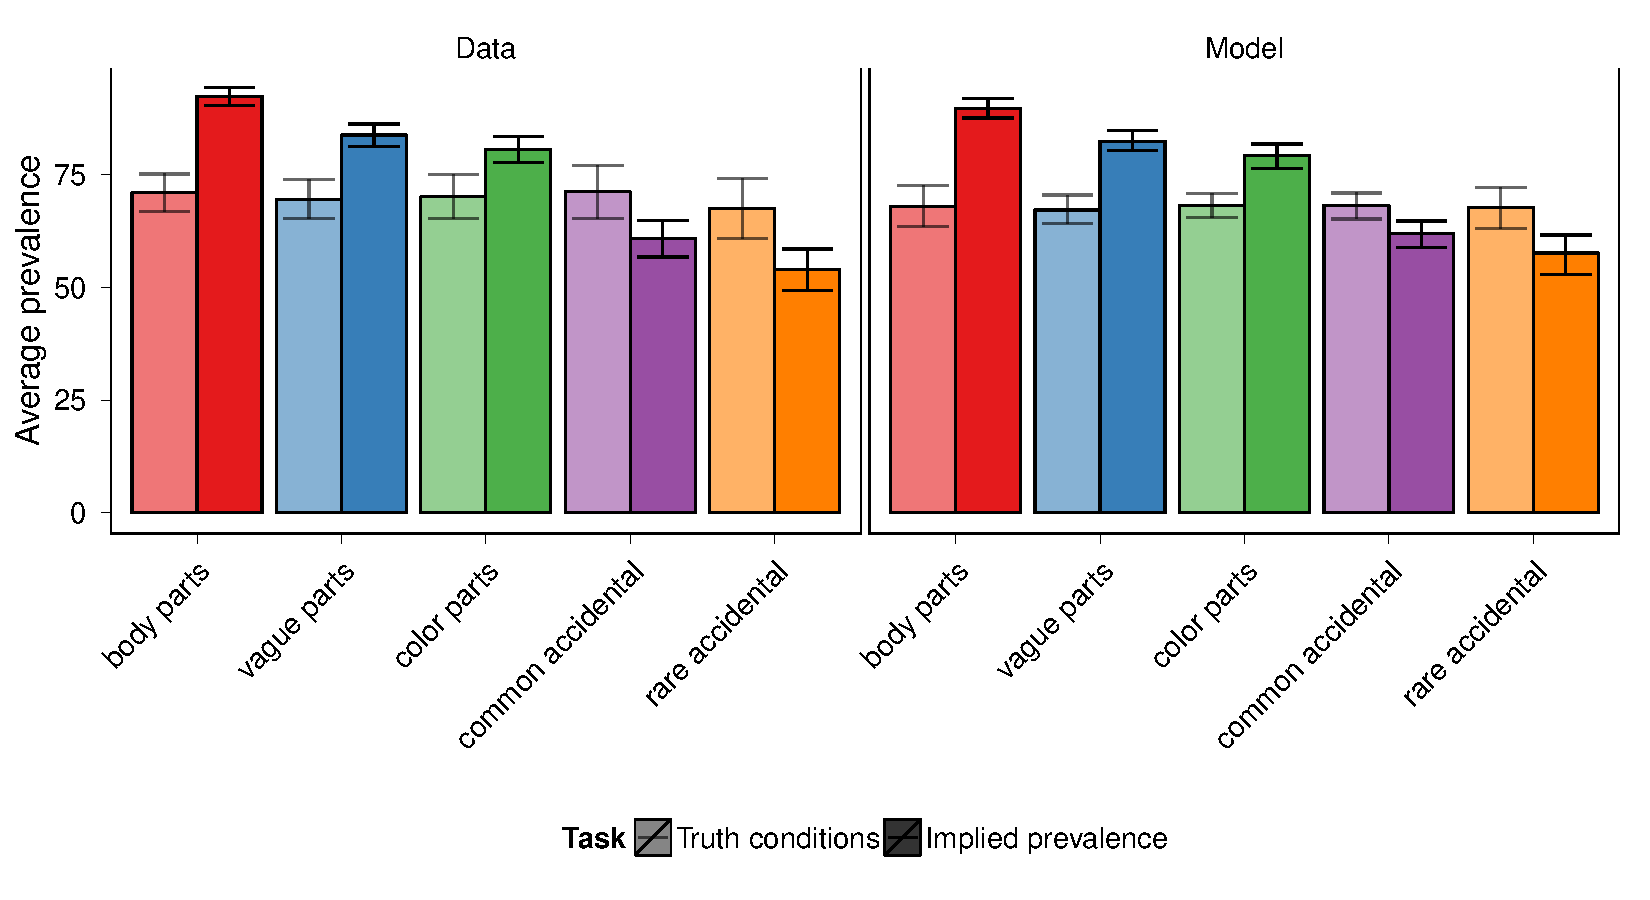
\includegraphics[width=\columnwidth]{asym-data-model-2opts-phi-100k.pdf}
    \caption{Replication and extension of \protect\citeA{Cimpian2010} (Left) and model predictions (Right). 
    Generic statements are accepted for a range of prevalences, resulting in an intermediate average prevalence (light bars) for ``truth conditions''. 
    Upon hearing a generic statement about biological properties, participants' infer that a high proportion of the category has the property (dark bars: red, blue and green). 
    Generics about accidental properties do not result in such a high implied prevalence (dark bars: purple and orange).  Error bars denote bootstrapped 95\% confidence intervals for the data and Bayesian 95\% credible intervals for the model.}
  \label{fig:exp2b}
\end{figure}


%
%Our results replicated the finding of CBG that the generic statements were endorsed more with dangerous and distinctive properties than with plain properties (Figure \ref{fig:exp1}, left; $\beta=1.99; SE = .36; z = 5.52; p < .001$). 
%%
%There was also an interaction between prevalence level and type such that the generic was endorsed more with \emph{dangerous and distinctive} properties than with plain properties at lower prevalence levels ($\beta=.03; SE = .01; z=2.35; p = 0.019$). There was a trending effect for the \emph{nondangerous and nondistinct} properties to be endorsed \emph{less} than the plain properties ($\beta=-.57; SE = .30; z=-1.91; p = .056$).

Implied prevalence of the generic was affected by the type of property in question (Figure \ref{fig:exp2b} Left; dark bars). 
Of theoretical interest is whether or not the median split we performed on the accidental properties based on the results of the prior elicitation experiment resulted in different implications for the associated generic.
We observe  greater implied prevalence of common accidental properties than rare accidental properties ($\beta=0.061; SE = 0.025; t(39) = 2.47; p = 0.018$ \footnote{These statistics are the result of a mixed-effects linear regression with a maximal mixed-effect structure: Random by-participant effects of intercept and slope}).
Implications of generics of body parts was significantly greater than those of the biological properties used by \citeA{Cimpian2010} (here, ``color parts'') ($\beta=0.118; SE = 0.024; t(39) = 4.74; p < 0.001$).
There was also a trending effect for the implications of vague body parts (e.g. curly fur) to be greater than those of color parts (e.g. yellow fur) ($\beta=0.032; SE = 0.016, t(54.8) = 1.95; p = 0.056$).


%The prevalence scores from each task were entered into a linear mixed model with a by-participant random effect of intercept; the fixed effects were property-type, task, and their interaction. Our results replicated the asymmetry finding that the generic statement was interpreted as having a higher prevalence than its truth conditions entail (i.e. main effect of task; $\beta=28.8; SE = 4.3; t=6.6; p < 0.001$; see Fig.~\ref{fig:exp2a}, right).

\subsubsection{Lifted-threshold model predictions}

In Expt.~1, the acceptability of the generic was modeled as a speaker (Eq.~\ref{eq:S2}) reasoning about whether or not to produce the generic given some known prevalence. 
We use the same model to make predictions for the \emph{truth conditions} data.
The \emph{implied prevalence} task is slightly different: Here, the participant hears a generic and is asked to infer the likely prevalence of the property. 
This is the model of the listener in Eq.~\ref{eq:L1}. 
We use this model to predict the data from the implied prevalence task.

Each of these models has a parameter governing the optimality of the hypothetical speaker in Eq.~\ref{eq:S1}. 
Since the supports of the distributions produced by the two models are different ($S_2$ returns a distribution over ``agree'' and ``disagree'', whereas $L_1$ generates a distribution prevalence levels), there is no reason to believe the speaker optimality parameters would be the same for the two models. 
Hence, we put independent prior distributions over the two parameters: $\lambda_{\text{truth conditions}}, \lambda_{\text{implied prevalence}} \sim \text{Uniform}(0, 20)$.

We model the observed data as being generated by a mixture of our generics model and a model of random guessing behavior. 
Modeling random guessing explicitly is important for recovering reliable estimates of the parameters of the model, which would otherwise be contaminated by this data \cite{LW2014}.
We put an uniformative prior over this mixture parameter $\phi \sim \text{Uniform}(0,1)$, and infer its credible values from the data.

\paragraph{Posteriors over model parameters}

To learn about the \emph{a posteriori} credible values of our model parameters, we used the probabilistic programming language WebPPL \cite{dippl} to collect 100,000 samples using the Metropolis-Hastings algorithm. 
The estimated posterior distribution of the contamination parameter $\phi$ parameter is shown in Figure \ref{fig:phi2}. 
This parameter represents the proportion of the data that is better explained by a model of random guessing than by the prevalence-based generics model. 
The 95\% Credible interval is [0.06, 0.15]. 

\begin{figure}
\centering
    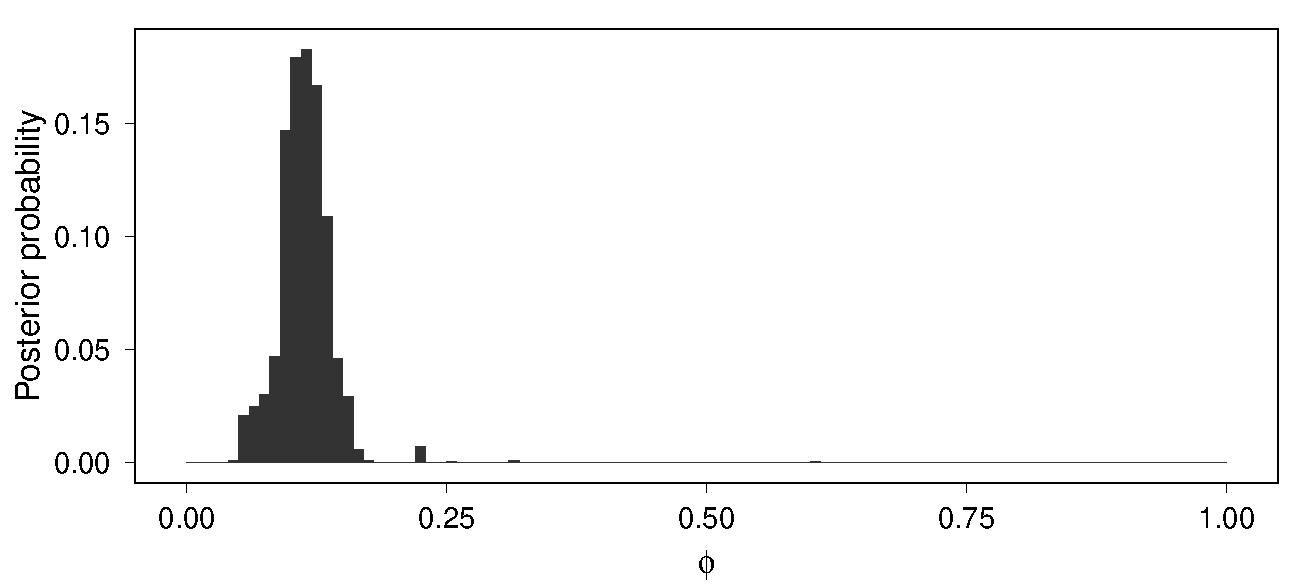
\includegraphics[width=0.8\columnwidth]{asym-phi-2opts-phi-100k.pdf}
    \caption{Posterior distribution of the contamination (``guessing'') parameter. The 95\% credible interval is [0.06, 0.15].}
  \label{fig:phi2}
\end{figure}

The estimated posterior distribution of the speaker rationality parameters $\lambda_{\text{truth conditions}}$ and $\lambda_{\text{implied prevalence}}$ are shown in Figure \ref{fig:rationality2}. 
This parameter represents the belief in how rational the hypothetical speaker in Eq.~{ref:eqS1} is believed to be when choosing to say the generic (over saying nothing). 
The 95\% credible interval for $\lambda_{\text{truth conditions}}$ is [0.23, 6.9] and $\lambda_{\text{implied prevalence}}$ is [1.30, 16.86]. The fact that these parameters are so different is expected given that the state space in the two tasks is also quite different.


\begin{figure}
\centering
    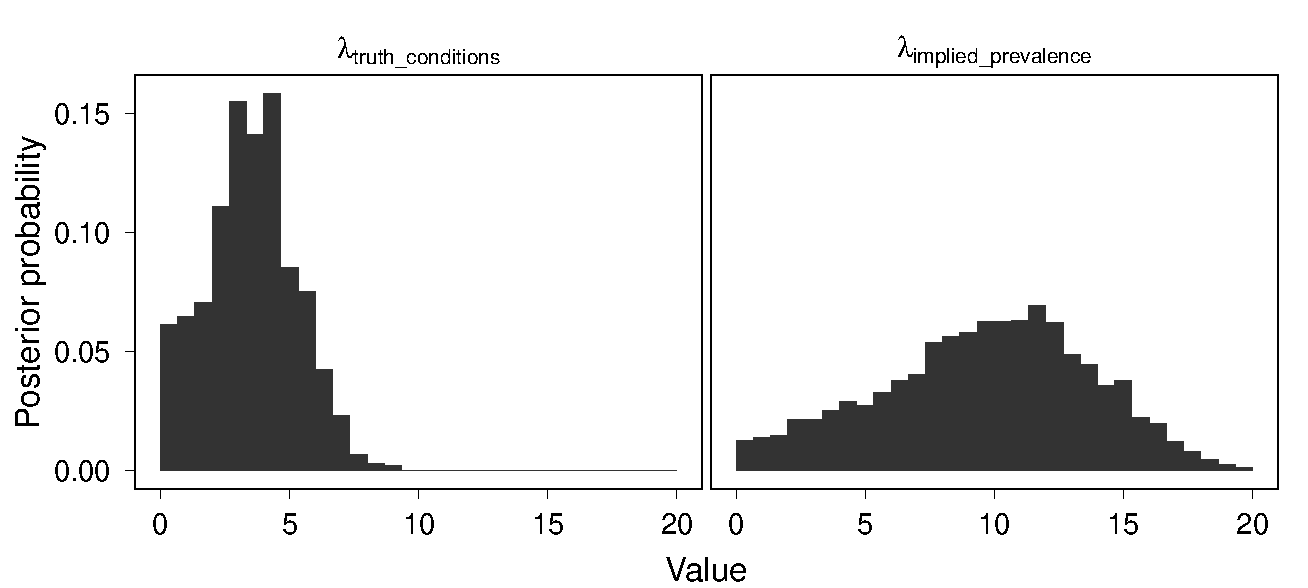
\includegraphics[width=0.8\columnwidth]{asym-lambdas-2opts-phi-100k.pdf}
    \caption{Posterior distribution of the speaker rationality parameters. The 95\% credible interval for $\lambda_{\text{truth conditions}}$ is [0.23, 6.9] and  $\lambda_{\text{implied prevalence}}$ is [1.30, 16.86]. The fact that these parameters are so different is expected given that the state space in the two tasks is also quite different.}
  \label{fig:rationality2}
\end{figure}

\paragraph{Posterior predictive}

The posterior predictive distribution is shown in Figure \ref{fig:exp2b} (Right). 
To generate the average truth conditions (light bars), we submitted our model to the same analysis as the data. We sampled the probability of accepting the generic for each prevalence level from the posterior predictive distribution. We then simulated a trial for each of the prevalence levels, and took the average prevalence level to which the model accepted the generic. We simulated 40 participants this way, and repeated the procedure 100 times to generate confidence intervals. The model shows an increasing endorsement of the generic as a function of prevalence (not shown), resulting in an intermediate but above 50\% average prevalence of acceptance. There were no appreciable differences between the average truth conditions among these properties. The implications of generics differ based on the type of property under discussion (Figure \ref{fig:exp2b}, Right, dark bars). We reproduce the behavioral data well ($r^2(10) = 0.97$). 


\subsubsection{Discussion}

To understand the behavior of the model, consider again the beliefs about the properties inferred from Expt.~2a (Figure \ref{fig:prior2}). 
All of the properties have substantial mass at 0 (Figure \ref{fig:prior2} Left). 
This gives the speaker validity in saying the generic at low prevalence levels (though his confidence in doing so increases as prevalence increases).
The listener has the complementary task: She brings \emph{a priori} uncertainty about the generic threshold to the table.
For illustration, consider what would happen if she inferred the most conservative threshold (0) and responded with the \emph{maximum a posteriori} (MAP) of the distribution. 
A threshold of 0 produces Figure \ref{fig:prior2} (right), because it only rules out the possibility that 0\% of the category has the property. 
The resulting peaks (MAPs) of the distributions are near 1 for biological properties (parts, color parts, vague parts) and around 10\% for accidental properties (both rare and common). This alone would produce variable interpretations. 
Our listener, however, does something wiser: She integrates over her uncertainty about the threshold (believing the speaker to be both truthful and informative), and produces implications that both take into account the peaks and the shapes of the resulting distributions.
This results in subtle differences between the implications of body parts (e.g. ``Glippets have wings.'') and  color parts (e.g.``Glippets have purple wings.''). 



\section{General discussion}

The lifted-threshold RSA model presented in this paper takes a generic statement to be vague. ``K has F'' means ``many members of K have F, \emph{relative to other categories, the vast majority of which, very few or none of the individuals in those categories have F}''. 
The model predicts a range of truth judgments for generics that seem to not have to do with prevalence. 
By considering not only the prevalence within the category but prevalence across categories, the model is able to arrive at graded and property-sensitive predictions about the truth judgments of generic statements, as seen in Expt.~1. 
The model very naturally accounts for the parallel problem of generic interpretation. 
Different \emph{a priori} beliefs about the distributions of properties both within- and across-categories give rise the puzzling asymmetries in how generics are interpreted relative to what is needed to felicitously use the generic. 

%This work speaks to a number of outstanding issues in psychology and linguistics. 

%On the linguistics end, w
We present a context-invariant semantics for generic statements. 
The stable meaning of a generic is as simple as possible: a threshold on prevalence, where the threshold is uncertain \emph{a priori} and only resolved by pragmatic reasoning.
This simple semantics is consistent with the profound phenomenon from cognitive development: Generics are learned at a very young age \cite{Gelman1998, Gelman2004, Gelman2008, Cimpian2008}.

We have explained two outstanding puzzles in language understanding. 
The first is that generic utterances can be true for a wide range of prevalence levels: from tigers with stripes all the way down to mosquitos with West Nile Virus. 
How can the prevalence of the property alone explain what makes some generics good things to say and others not as good? 
The insight is that with an uncertain semantics, the likely meaning of the generic (i.e. the likely threshold for acceptance) is inferred using listeners' \emph{a priori} beliefs and the communicative force of a speech act. 
This leads to different thresholds for different types of properties. 

The second phenomenon is the generic utterances often carry strong implications, though not all bare plurals have this impact. 
We measured participants' beliefs about the distributions of properties and found the accidental properties are utterly distinct in shape from biological properties.
Biological properties are characterized by \emph{widespread prevalence}, even though they may be rare across kinds (e.g. purple feathers).
Accidental properties, by contrast, are both rare across and within kinds: \emph{broken legs} are \emph{a priori} most likely to present in a small fraction of the population.
Thus, when given a vague utterance in the form a generic, the most likely \emph{a posteriori} prevalences vary in ways that match human participants' intuitions about the implied prevalence.


\subsection{Conceptual distinctions and prevalence}

We have shown that the truth conditions and implications of generics can be explained by beliefs about the prevalence of properties within- and across- categories. 
However, there is an open question of where \emph{these distributions} come from. 
It is quite plausible that these distributions are derived from higher-order conceptual knowledge about the nature of these properties \cite{Gelman2005, Keil1992}.

In Expt.~1a, participants estimated the prevalence of properties for many different kinds of animals. This was aggregated to form a distribution of prevalence across kinds.
In Expt.~2a, we measured this distribution by sequentially asking questions at different levels of abstraction: Question 1 was about the prevalence across categories while Question 2 was about prevalence within categories. 
It is likely that further abstracting the problem to more conceptual level questions (e.g. ``Are there differences between male and female lorches?''; ``Do you think a young fep is likely to have long legs?'') would elucidate the connection between distributions on prevalence and conceptual representations. 

Much of the psychological and philosophical work has looked beyond prevalence and focused on conceptual distinctions among generics \cite{Prasada2013, Leslie2008}. For example, \citeauthor{Prasada2013} has argued for a distinction between \emph{characteristic} properties (e.g. ``Diapers are absorbent.'') and \emph{statistical} properties (e.g. ``Diapers are white.''). Where in the prevalence-based semantics could such conceptual distinctions come into play?

Probabilistic models are a useful way to represent rich, structured knowledge of world \cite{Goodmanconcepts}. It's plausible that the prevalence distribution we've focused on in this work is actually derived from richer conceptual knowledge. For the purpose of the semantics of generics, this work shows that prevalence is sufficient to capture the range of truth judgments for these sentences. How a listener arrives at an estimate of the prevalence, or the prevalence distribution at large, may be the result of a probabilistic, conceptual model of the world. 

It's important to stress that our approach puts at its core listeners' \emph{beliefs} about the prevalence of the properties in question. 
Our participants' estimated the prevalence of certain properties to be much higher than the actual statistics of the world \red(example?).
This is an important methodological contrast to what is often employed in semantic approaches to generics, that prevalence is about \emph{actual prevalence in the world}. 
Along similar lines, this work used utterances about animal kinds in these experiments because participants' beliefs about these properties and categories are likely to be relatively homogenous (thus, lower noise). However, generic language is often used in everyday conversation to talk about social categories: In these domains, we would expect large individual differences in generic acceptability and interpretations.


An additional issue, one that likely interacts with conceptual distinctions, is how to determine the kinds of things against which a speaker implicitly compares the prevalence of the category in question. Here, we have used only generic sentences about animals, where the likely contrast class is other animals (e.g. ``Mosquitos carry malaria, \emph{relative to other kinds of living creatures}''). Moving outside the domain of animals, the makeup of this contrast class becomes less clear. 


A further observation concerning the nature of this contrast class is that focus, as a result of prosodic cues for example, can change the distribution against which one compares the prevalence of a property. For example, is a person asks ``What carries malaria?'', a very natural answer would be ``MOSQUITOS carry malaria'', since Mosquitos more than any other animal kind carry malaria. By contrast, if a person asks ``What are mosquitos like?'', is it natural to reply ``Mosquitos CARRY MALARIA''? 
Our suspicion is that it is not as natural because of salient alternatives (``Mosquitos bite you'', ``Mosquitos suck blood.'', ``Mosquitos make buzzing sounds''). 
Here, the contrast class is not with respect to \emph{other animals} but with respect to other properties \emph{of that animal}. 
Notice, however, that the underlying dimension that these properties would be compared along is still prevalence. What has changed is what constitutes this distribution: prevalence across categories vs. prevalence across properties.



%We used a Bayesian data analytic model to make a ``backward prediction'' about the underlying prevalence prior by way of the observed experimental generics data and the lifted-threshold RSA model. We verified this prediction and then incorporated the empirical prior into the model, reconfirming the original fit. We showed how our model predicts a dissipation (or even reversal) of the asymmetry between truth conditions and implications of generics as first explored by \citeA{Cimpian2010}. Finally, we explored how far prevalence alone could take us, by measuring the prior for just \emph{dangerous} properties. We found that while \emph{dangerous} properties were interpreted as more distinctive and plain properties, this difference only led to marginal increases in the predicted ``true'' responses in the truth conditions task. 
%
%The observation that the predictions for the truth conditions task were \emph{qualitatively} correct but \emph{quantitatively} not as large as the observed behavior data gives rise to at least two possible explanations. First, it is possible that our technique for measuring the prior distribution over prevalence is too crude to account for such small differences in prevalence. It was not guaranteed that differences in the truth conditions tasks between truth judgments at different prevalence levels would actually show up as important differences in the prior elicitation task. 
%Additionally, the measurements made in the truth conditions task might also be too coarse: In these experiments, truth conditions are measured by categorical judgments (\emph{true} or \emph{false}) at prevalence intervals of 20\%. It's possible that more graded judgments at finer prevalence scales would be helpful in mediating this. However, it's also possible that with an uncertain threshold for the generics, participants will adapt to whatever prevalence sampling an experimenter presents. At the end of the day, the truth conditions task is interested in measuring the prevalence level at which the generic is true. It's likely that other, convergent measures would be helpful in assessing this. 
%
%A second possibility for the seeming failure to account for the magnitude of the effect in truth judgments for different property types is because prevalence alone is not being used as the only measuring stick for assessing the generic. It's possible that something about the salience of the property (e.g. instantiated in its dangerousness) leads ones to be more flexible in its usage\cite{Leslie2008}. This explanation could be cashed out in a model of nonliteral language like the one in presented by \citeA{Kao2014}. The idea here would be that using a generic to describe a salient (e.g. dangerous) property of a kind would be like using hyperbolic language. This type of generic, then, would convey the idea of prevalence in addition to an affective message, like ``be careful''. We leave for future work exploring this type of explanation in more detail.
\subsection{What are generics?}

Intuitions about what qualifies as a generic statement have led to the consensus that there are generic and non-generic meanings that can be derived from similar syntactic forms. For example,
\begin{quotation}
	(1) Tigers are massive. 
	
	(2) Tigers are on the front lawn.
\end{quotation}

Classically, (1) is understood as referring to the kind whereas (2) is understood as referring to a plurality of instances. 

In our follow-up to \citeauthor{Cimpian2010}'s study on the implied prevalence of generic statements about accidental properties, we found a gradient of implied prevalence, which was driven by listener's \emph{a priori} beliefs about the prevalence of the property. 
The finding that different properties receive variable interpretations suggests a categorical distinction between generic and non-generic bare plurals may not be necessary. 
Consider the following 

\begin{quotation}
	(3) Tigers are on front lawns. 
	
	(4) Tigers are in zoos.
	
	(5) Tigers are in open grasslands.
\end{quotation}

It seems that as you go from (3) - (5), the likely implied prevalence also increases, to the point where (5) might apply to category as a whole. 
With a generic whose meaning is vague, as we propose here, listeners need not make categorical distinctions to interpret a sentence. 
Rather, they only need consult their beliefs about the properties in question to resolve reasonable interpretations. 

\subsection{Vagueness and communication}

We have presented a semantics for generics in which they convey a threshold on prevalence which is uncertain but fixed through pragmatic reasoning about the distribution of prevalence for the property in question.
In Expt.~2a, we showed how this prevalence distribution can be elicited by sequentially asking about the prevalence across- and within- categories. 
Within-category prevalence was elicited by asking a question about generalization: ``Imagine there is a glippet that has green legs. What \% of glippets do you think have green legs?''.

The model of generic communication that we've introduced uses a threshold whose value is uncertain. 
In a sense, the bare minimum that the generic communicates is that we are in a situation where there is a glippet that has green legs. 
The listener then is then left to her own devices to generalize as widely as she deems based on her beliefs about the property. 
This is consistent with the notion of a GEN operator that tells the listener to generalize this fact \cite{Leslie2008}.


The generic, it seems, doesn't convey any additional information beyond what the listener already knew about the prevalence of the property.
This shouldn't surprise us. ``John is tall'' does not actually tell us about what \emph{tall} means\footnote{However, ``John is a person'' does tell a listener about what \emph{tall} means in ``John is tall''.}. 
Rather, the listener is expected to come to the conversation with some beliefs about heights, and knowing that John is a person, be able to infer likely meanings for \emph{tall}.
%In exactly the same way, a speaker uttering ``Glippets have green legs.'' doesn't tell the listener 






%
%\subsection{Resilience to counter-examples}
%
%\subsection{A parallel problem of generic identification}


% on the problem of generic meaning, using sentences with bare plural construction. The bare plural construction is likely the easiest to interpret generically. For example, in the work of \citeA{Prasada2013}, the overall ``true'' responses for statements in the bare plural construction (regardless of content) was appreciably higher than all other sorts of constructions associated with generic meaning. Bare plurals are easily read generically. 

%Stepping outside of bare plurals, one runs into a problem parallel to that of generic meaning: generic identification. For example, ``Tigers are ferocious'' can be read generically whereas ``Tigers are on the front lawn'' cannot. Sensitivity to contextual and morphosyntactic cues begins early on \cite{Cimpian2008}. 



%\subsection{Generics in learning}
%
%In this work, we have found that differences in the distributions of prevalence can explain differences in truth conditions for different types of properties. 
%An open question for this line of work is how do listeners come to have different priors for different property types in the first place? 
%It's estimated that generics account for 4\% of all utterances addressed to preschool-age children in everyday contexts \cite{Gelman2008} and that 2-3 year old children comprehend generic statements \cite{Cimpian2011, Gelman2003}. 
%If interpreting a generic requires knowledge about the distribution of the prevalence of the property, where do children learn that from? 
%One possibility is that they learn it at the same time that they learn the meaning of the word \cite{Frank2009}. Further work should explore the learning problem in terms of a joint inference about the possible category in reference and the still-being-learned meaning of words. 
% 
\subsection{Conclusion} 


We have explored and demonstrated the viability of a scalar semantics for generics when coupled with a sophisticated pragmatics. 
A lower-bound threshold on prevalence---the probability of the property given the category---is inferred as part of pragmatic interpretation, yielding vague and context sensitive meanings. 
%We first used Bayesian data analysis to show that the effective threshold of a fixed-threshold semantics would need to vary by context, and yet it still not account adequately for the data. 
%
%
We formalized reasoning about the threshold in a lifted-threshold Rational Speech Acts model. This model predicted graded truth judgements and an asymmetry between truth and prevalence judgments. It also naturally accommodates the role of context, explaining these effects as the result of variation in the prevalence prior. 

Generics are ubiquitous in natural language. It might seem paradoxical, then, that the semantics of generic statements are underspecified. Why should vague language get so much usage? One possibility is apparent in the lifted-variable RSA model: generic language provides interlocutors with the flexibility to convey meanings as rich as our conceptual knowledge. %, which are easily understood in context. 
Generics are vague, but predictable and useful.


%In Experiment 2, we verified that participants' beliefs about the prior on prevalence varied in this way. 
%This provides evidence that the model we propose can account for many of the empirical phenomena associated with generics.

%We have shown how a Bayesian model of language understanding, motivated by contextual variation of the effective threshold of the generic statement, can explain the puzzling truth conditions and asymmetrical meanings of generic language. We have used techniques in Bayesian data analysis to help arbitrate between two cognitive theories. The first was a simple theory that proposed that a generic was akin to some alien quantifier. In this theory, the generic behaves like other quantifiers in that it has a fixed-threshold semantics. We explored one elaboration of this in allowing the generic to have a threshold that differed across contexts. 
%
%The alternative theory is that there is no generic threshold out there in the world to observe. Instead, listeners infer the threshold (and thus, the semantic content) of the words from context. The posterior predictive distributions of the lvRSA model account for the contextual variation in the generic endorsements, both quantitatively and qualitiative. It further accounts for the asymmetry between verification and interpretation by considering different Questions Under Discussion (QUDs) and communicative roles (speaker / listener) in the two tasks. Finally, the Bayesian analytic techniques allowed us to make a new prediction as to the shape of the prior distribution over prevalence levels for different contexts. Exp. 2 found confirmatory evidence that this is indeed how people think these properties are distributed.

%\section{Further simulations}
%
%Our model makes the prediction that if the shape of the prior distribution was not bimodal, the asymmetry between verification and interpretation would change. Indeed, this is a similar prediction to \citeA{Cimpian2010}, who posited that accidental or disease states (e.g. ``muddy feathers'', ``infected ears'') would weaken the asymmetry. We would expect accidental or disease states to not follow a bimodal distribution. 
 




%\begin{itemize}
%
%\item Replace figure 4 (hyperprior parameters) with mean distribution?
%
%\item Collapse Figure 3 \& 5 (posterior predictive) into one
%
%\item Exp 2 to confirm $\gamma$ and $\delta$. 
%
%\item Some linking function to condition on Exp 1 \& 2 simultaneously,  to perhaps, infer rationality parameter and get some posterior predictives.
%
%\end{itemize}
%
%The data analysis involved comparing the mean of the prevalence ratings associated with \emph{True} endorsements of the generic with the mean prevalence ratings elicited by the generic in a separate task. In the experimental pragmatics literature, the dependent measure involved in the ``truth conditions'' task is called \emph{sentence verification}; in the ``implied prevalence'' task, it is a \emph{sentence interpretation}. 
%
%These different dependent measures, we argue, imply different Questions Under Discussion (QUD, \cite{Roberts2004}). 



%	\section{Sentence verification is a speaker task}
%	
%	DegenGoodman2014.  Truth conditions task --> QUD = ``generic true?'' Model.
%	
%	But what is the semantics of the generic? \citeA{Cimpian2010}, experiments 1, 3, and 4 found that the truth conditions of the generic are sensitive to the context.  Our goal is to replicate this finding, and use Bayesian data analysis to infer the threshold of the speaker model. This bears some similarity to Michael Franke's approach for cogsci from last year.
%	
%	
%	
%	
%	\section{The full bayesian thing}
%	
%	Computational models of cognition typically have parameters. Many of these parameters are of theoretically interest, because they are posited to reside within the head of the subject.
%	
%	\subsection{Inferring quantifier threshold by context}
%	
%	Here we'll find that the generic threshold changes by context. We might also want to show that ``most'' and ``some'' do not change by context.
%	
%	\subsection{Are generics like adjectives?}
%	
%	To determine if a generic is true or false, we must refer to context. The threshold in the threshold-semantic view of the statement varies by context. This property has been shown to be an important feature in the semantics of gradable adjectives (e.g. \emph{tall}) \cite{Lassiter2014}.  
%	
%	\section{Lifted-variable speech act model}
%	
%	We can start in a single context, with a uniform prior over states. We can look at the posterior over states, for listener1. As well, we can look at the posterior over thetas. This depends of course on the alternatives, for which we may want to consider only the experimental alternatives \emph{some, most, generic} or for which we may want to include \emph{all}.  Either way, here we'll recreate the asymmetry between listener and speaker --- between implied prevalence and truth conditions. 
%	
%	\citeA{Cimpian2010} report a ``paradoxical asymmetry at the core of generic meaning'' which manifests as the generic having ``extremely strong implications but requiring little evidence to be judged true''. Here, we explain this ``paradox'' by the different Questions Under Discussions in the tasks used and by the different roles intrinsic to speech-acts: the role of the speaker and the role of the listener. 
%	
%	\subsection{Questions Under Discussion in two tasks}
%	
%	\citeA{Cimpian2010} used two tasks (with different dependent measures) to get at the comparison between ``acceptance'' and ``implications''. These two tasks --- called ``truth conditions'' and ``implied prevalence'' -- used different questions and different dependent measures to get at the meaning of generics. In the ``truth conditions'' task, subjects are given evidence about the prevalence of a property (e.g. ``50\% of morseths have silver fur'') and are asked to judge the corresponding generic (i.e. ``Morseths have silver fur'') to be either true or false. In the ``implied prevalence'' task, subjects are given a generic statement and asked ``What percentage of morseths do you think have silver fur?''
%	
%	\citeA{Degen2014} argue that the \emph{sentence verification} (``truth conditions'') task should be modeled as a speaker task, and that the \emph{sentence interpretation} (``implied prevalence'') task should be modeled as a listener task. In addition to different communicative roles, there are also different implicit Questions Under Discusision. In the ``truth conditions'' task, the QUD seems to be ``is the generic true or false?'', whereas in the ``implied prevalence'' task, the QUD seems to be ``what percentage of category X have property Y?''.



\appendix
\section{Stimuli used in Experiment 1}
\label{sec:appendix}	

\begin{table}[h]
\begin{tabular}{| l || l | l | l |}
\hline
Conceptual type               & Item                    & Truth judgment & Prevalence estimate \\
\hline \hline
Majority characteristic       & 1. Leopards have spots.    &                &                     \\
                                          & 2. Ducks have wings.                       &                &                     \\
                                          & 3. Cardinals are red.                       &                &                     \\
                                          & 4. Swans are white.                       &                &                     \\
Minority characteristic       & 5. Lions have manes.       &                &                     \\
                                          & 6. Kangaroos have pouches.                        &                &                     \\
                                          & 7. Robins lay eggs.                        &                &                     \\
Striking                      & 8. Sharks attack swimmers. &                &                     \\
                                  & 9. Mosquitos carry malaria.                        &                &                     \\
                                  & 10. Ticks carry lyme disease.                        &                &                     \\
                                  & 11. Tigers eat people.                        &                &                     \\
Majority false generalization & 12. Robins are female.      &                &                     \\
                                              & 13.  Lions are male.                       &                &                     \\
False                         & 14. Leopards have wings.       &                &                    \\
                                              & 15. Kangaroos have spots.                       &                &                     \\
                                              & 16.  Tigers have pouches.                       &                &                     \\
                                              & 17.  Robins carry malaria.                       &                &                     \\
                                              & 18. Sharks have manes.                       &                &                     \\
                                              & 19. Lions lay eggs.                       &                &                     \\
                                              & 20. Swans attack swimmers.                       &                &                     \\
Novel                         & 21. Mosquitos attack swimmers.       &                &                    \\
                         & 22. Sharks lay eggs.       &                &                    \\
                         & 23. Frogs have spots.       &                &                   \\
\hline

\end{tabular}
\caption{Stimuli used in Experiment 1.}
\label{tab:expt1}
\end{table}


\section{Instructions used in Experiment 1a: prior elicitation for familiar categories}
\label{sec:prior1instruct}

Participants were told 
\begin{quote}
In this study, we are interested in how prevalent certain properties are within different kinds of animals. We will give you examples of the kinds of animals we have in mind and ask you to list a few of your own.

Then, you will estimate the \emph{percentage of the individual members} of the animal species that have certain properties.

On each trial, you will rate 8 properties. The properties will be revealed to you one at a time. Essentially, you will be filling out a big table. You are allowed to go back and revise your answers, if you think there is a more realistic estimate you could give. You will do this 2 times (2 big tables). 

\end{quote}


\section{Instructions used in Experiment 2a: prior elicitation for novel categories}
\label{sec:prior2instruct}

Participants were again told they were on a newly discovered island with lots of new animals on it. They were then given the following instructions

\begin{quote}
One day, you are roaming through the library when you encounter a data-collection robot. The robot doesn't know very much about the world and is asking you questions to learn more. Today, it wants to learn about properties of animals. It is randomly selecting an animal from its memory and a property from its memory, and asking you if the animal is likely to have the property.

Of course, you're new to this island so you don't really know anything about these animals. The properties, however, will be familiar. Try to provide your best guess given your own experience.
\end{quote}

Participants were then run through a practice trial where they were familiarized with the questions that would be asked on them. 
On each trial, the data-collection robot introduced a new animal (e.g. ``We recently discovered animals called glippets.''). 
The robot then asked how likely it was that ``there was \emph{a} glippet with [[property]]''. 
This question aimed to get at the prevalence of the property \emph{across} categories (e.g. it's very likely that there is a glippet that is female, less likely that there is a glippet that has wings, and even less likely that there is a glippet has purple wings). 
The second question was about the prevalence \emph{within} categories. The robot asked, ``Suppose there is a glippet that has wings. What percentage of glippets do you think have wings?''

\section{Stimuli used in Experiment 2}
\label{sec:materials2}

Many of these materials were originally used in \citeA{Cimpian2010}.

\begin{table}[h]
\begin{tabular}{| l || l | l | l |}
\hline
Property type               & Item                    & Across-category prevalence estimate  & Within-category prevalence estimate \\
\hline \hline
Body part       			& 1. Teeth    &   &                     \\
                                          & 2. Fur                       &                &                     \\
                                          & 3. Tails                     &                &                     \\
                                          & 4. Claws                       &                &                     \\
                                          & 5. Feathers                       &                &                     \\
                                          & 6. Ears                       &                &                     \\
                                          & 7. Legs                       &                &                     \\
                                          & 8. Skin                       &                &                     \\
Colored part      	 & 9. Pink teeth       &                &                     \\
                                          & 10. Yellow fur                       &                &                     \\
                                          & 11. Orange tails                         &                &                     \\
                                          & 12. Blue claws                       &                &                     \\
                                          & 13. Purple feathers                      &                &                     \\
                                          & 14. Orange ears                    &                &                     \\
                                          & 15. Silver legs                       &                &                     \\
                                          & 16. Violet skin                      &                &                     \\       
Vague part      	 & 17. Long teeth       &                &                     \\
                                          & 18. Curly fur                       &                &                     \\
                                          & 19. Long tails                         &                &                     \\
                                          & 20. Big claws                       &                &                     \\
                                          & 21. Smooth feathers                      &                &                     \\
                                          & 22. Small ears                    &                &                     \\
                                          & 23. Long legs                       &                &                     \\
                                          & 24. Rough skin                      &                &                     \\ 
Common accidental part    & 25. Wet fur       &                &                     \\
                                          & 26. Dusty skin                       &                &                     \\
                                          & 27. Worn-out claws                         &                &                     \\
                                          & 28. Fungus-covered fur                      &                &                     \\
                                          & 29. Muddy feathers                      &                &                     \\
                                          & 30. Rotten teeth                   &                &                     \\
                                          & 31. Torn feathers                       &                &                     \\
                                          & 32. Itchy tails                      &                &                     \\  
Rare accidental part    & 33. Sore legs       &                &                     \\
                                          & 34. Torn tails                       &                &                     \\
                                          & 35. Cracked claws                         &                &                     \\
                                          & 36. Sore teeth                       &                &                     \\
                                          & 37. Swollen ears                      &                &                     \\
                                          & 38. Infected ears                    &                &                     \\
                                          & 39. Burned skin                       &                &                     \\
                                          & 40. Broken legs                     &                &                     \\                                                                                          
                                           \hline

\end{tabular}
\end{table}



\bibliographystyle{apacite}

\setlength{\bibleftmargin}{.125in}
\setlength{\bibindent}{-\bibleftmargin}

\bibliography{generics}


\end{document}


% after cogsci
% prior elicitation for accidental / disease states
% -- asymmetry weakened

% most / some: better experiments
% -- asymmetry X prior analysis

